\chapter{Water level Prediction based on High-resolution Synthetic Aperture Radar Images}
\label{chap-5-predict-from-sar-image}
\begin{ChapAbstract}
In this chapter, we would like to apply machine learning approach, especially deep learning, to predict the water body in the next future. We apply an extension on Long Short-Term Memory (LSTM), Conv-LSTM, to tackle problem. Conv-LSTM layer is not only take advantage from previous state-of-the-art approach in this kind of problems, Fully-Connected LSTM, but also very suitable to spatial-temporal data due to inherent convolutional structure. Because the common information that we can accquired from water body and rainfall intensity, are spatial and temporal, we apply model from precipitation nowcasting problem to our prediction problem, modify about ways to train model, then Tri An Reservor is one more time selected to take experiment on. 

\end{ChapAbstract}

\section{Introduction}

% Time-series data prediction: Video / Precipitation Nowcasting.

Prediction (a.k.a. sequence prediction) is one of interesting fields in machine learning, in which the input (sequence data) contains an order on the observations and this order must be preserved while training model and making prediction.

\begin{figure}[h!]
	\centering
	\includegraphics[width=0.7\textwidth]{figures/Example-of-a-Sequence-Prediction-Problem.png}
	\caption[]{Example of simple sequence prediction}
	\label{fig:exampleSimpleSequencePrediction}
\end{figure}

There are some example of sequence prediction problems, including:

\begin{enumerate}
	\item \textbf{Stock Market Prediction}\cite{Pagolu2016,Liu2018}. Given sequence of stock value as input, predict the expected next stock value. 
	
	\item \textbf{Product Recommendation}\cite{Wang2018,Cao2019}. Given sequence of recent purchased goods of a customer, predict the thing that the customer might "add to cart" next, and then make recommendation. 
	
	\item \textbf{Weather Forecasting}\cite{Quan2000,Wang2017}. Given sequence of weather observation over a period of time, predict the expected weather in next point of time.
	
\end{enumerate}

% Related to water body from satellite images, figure out why it related and its expansion: periodical information

One of important fields of weather forecasting is Nowcasting Precipitation\cite{Sun2013}. The goal of this task is about giving precise prediction of rainfall intensity in a region, over a short period of time. Recent advances in deep learning, Recurrent Neural Networks (RNNs), especially Long Short-Term Memories (LSTMs) models\cite{Graves2013GeneratingSW,Hochreiter1997,Cho2014,Donahue2017} provides good results on this kind of problem. In this chapter, we would like to predict the next water body shape (related to its area), from its time-series data. The common things between nowcasting precipitation and this problem is they both have spatial, spectral and temporal information inside data. We would like to apply model containing Conv-LSTM-2D layer\cite{Shi2015ConvolutionalLN}, to solve our proposed problem. Conv-LSTM-2D layer is recently used in computer vision, especially spatial-temporal problems. In this problem, we would like to extract the spatial feature as well as the correlation in the time. The fully-connected LSTMs can capture the temporal correlation but do not encode the spatial data. That's why they propose a model where the input to state and state to state transitions are convolutional. The model in \cite{Shi2015ConvolutionalLN} show better result on capturing spatial-temporal correlations than other state-of-the-art methods. So in this chapter, we will take this model as reference to provide solution for our problem, for Tri An reservoir.

\paragraph{Synthetic Aperture Radar (SAR) Images} \footnote{https://en.wikipedia.org/wiki/Synthetic-aperture\_radar} SAR is a form of radar, which mainly used to produce two or three-dimensional reconstructions of objects. SAR is motivated for high-resolution remote sensing and it is independent of weather. It also has many application in remote sensing, including topography, oceanography; environment monitoring such as oil spills, flooding, urban growth, global change and military surveillance and so on. 

\begin{figure}[h!]
	\centering
	\includegraphics[width=0.4\textwidth]{figures/TEIDE.jpg}
	\caption[]{Teide volcano on the island of Tenerife in the Canary Islands, Spaceborne Imaging Radar-C/X-Band Synthetic Aperture Radar.}
\end{figure}

\paragraph{Sentinel 1-A Satellites} The Sentinel-1 mission \footnote{https://sentinel.esa.int/web/sentinel/missions/sentinel-1} comprises a constellation of two polar-orbiting satellites, operating day and night, in order to acquire imagery regardless of the weather. This is one of big benefits when comparing with Landsat satellites. Launched on 3rd April 2014, Sentinel-1A is placed in a near-polar, sun-synchronous orbit with a 12-day repeat cycle and 175 orbits per cycle.

\section{Dataset} 

In this chapter, Tri An reservoir is chosen for experiments. Because Radar Satellites Images is not affected by cloud cover like optical satellite in \ref{chap-3-recover-water-body}, so we only focus on prediction water body. The SAR images monthly imagery provided from Sentinel-1 satellites are collected from \textit{November 25tr, 2015} to \textit{June 1st, 2019} for training and evaluating. 

Depending on coordinates of Tri An Reservoir, the original image has been cropped to size \textit{2560 px} x \textit{3840 px}, enough to show its water body.

\paragraph{Water body segmentation on Sentinel-1 Image} In this chapter, in order to segment out water body, we depend on \textbf{V}ertical Transmit-\textbf{H}orizontal Receive Polarization (VH) or \textbf{V}ertical Transmit-\textbf{V}ertical Receive Polarization (VV), and apply corresponding threshold:

\begin{equation}
\centering
VH \leq -21
\end{equation} 

\begin{equation}
\centering
VV \leq -17
\end{equation} 

\subparagraph{Polarization} Polarization is a way to give transmission signals a specific direction. It makes the beam more concentrated. Signals transmitted by satellite can be polarized in one of four different ways: linear (horizontal or vertical) or circular (left-hand or right-hand). To use the channels that are available for satellite broadcast as efficiently as possible, both horizontal and vertical polarization (and left- and right-hand circular polarization) can be applied simultaneously per channel or frequency. Horizontal and vertical transmissions will therefore not interfere with each another because they are differently polarized. This means twice as many programs can be transmitted per satellite. Consequently, via one and (almost) the same frequency the satellite can broadcast both a horizontal and a vertical polarized signal (H and V), or a left- and right-hand circular polarized signal (LH and RH).

\begin{itemize}
    \item \textbf{\textit{V}ertical Transmit-\textit{H}orizontal Receive Polarization (VH)} is a mode of radar polarization where the microwaves of the electric field are oriented in the vertical plane for signal transmission, and where the horizontally polarised electric field of the backscattered energy is received by the radar antenna.
    \item \textbf{\textit{V}ertical Transmit-\textit{V}ertical Receive Polarization (VV)} is a mode of radar polarization where the microwaves of the electric field are oriented in the vertical plane for both signal transmission and reception by means of a radar antenna. In this case, the plane of the electric field of the microwave energy is designated by the letter V (vertical) for both transmit and receive events, i.e. VV; this transmit-receive polarity is also called like-polarised as opposed to cross-polarised (horizontal transmit - vertical receive, HV). 
\end{itemize}

Because in our cropped image that only contains Tri An Reservoir as the largest water body, so we only need to find out the most largest one, using Bread-First Search algorithm\footnote{https://en.wikipedia.org/wiki/Breadth-first\_search}. With this object, we easily to figure out the boundaries, with help of function \textit{find\_boundaries}, from Python library \textit{Scikit-Image}\footnote{https://scikit-image.org/}.

% \pagebreak
\section{Model}

In this thesis, we stack Encoding-Forecasting Conv-LSTM layer to for building prediction model. Our input and output of model are all 3D tensors, size of $T x W x H$, in which $T = 12$ for temporal information (12 consecutive months), where $W x H$ is size of each data point image for spatial information. This helps our model preserve all spatial and temporal information, so that, it can tackle the complex water body prediction problem, with multiple stacked of Conv-LSTM-2D. In Figure \ref{fig:structureConvLSTM2D}, the encoding LSTM compresses, while the whole input sequence into a hidden state tensor and the forecasting LSTM unfolds this hidden state to give the final prediction.

\begin{figure}[h!]
	\centering
	\includegraphics[width=0.8\textwidth]{figures/convlstm_sample.PNG}
	\caption[]{Structure of Encoding-Forecasting Conv-LSTM network in \cite{Shi2015ConvolutionalLN}}
	\label{fig:structureConvLSTM2D}
\end{figure}

Conv-LSTM-2D is already provided in Keras framework\footnote{https://keras.io/layers/recurrent/}. Model structure is shown in Figure \ref{fig:timeModel}.

\begin{figure}[h!]
	\centering
	\includegraphics[width=0.4\textwidth]{figures/time_model.png}
	\caption[]{Prediction mode, based on Conv-LSTM-2D}
	\label{fig:timeModel}
\end{figure}

Specification:

\begin{itemize}
	\item \textit{Input and Output} Because we only focus on predicting water body, so after extracting water body from original image and finding out its boundaries, we randomize on boundaries 50 tiles with size of 128 x 128. There is 12 consecutive images, corresponding to 12 month in year. The output is a image of next month, which is same month of 1st image in input sequence but next year. 
	
	\item \textit{Conv3D} This type of layer helps to catch spatial and temporal invariances in the same manner as \textit{Conv2D} in an imagery case. This make the curse of dimensionality much less harmful. Because at the end of model, we need to have a prediction, so it's no longer to keep temporal information after this layer.
	
	\item \textit{Batch Normalization} Batch normalization reduces the amount by what the hidden unit values shift around (covariance shift). Morever, this layer allows each layer of a network to learn by itself a little bit more independently of other layers.
	
	\item \textit{Activation} The activation for Conv-LSTM-2D is $tanh$ function, for Conv3D is $sigmoid$ function.
	
	\item \textit{Dropout and Recurrent Dropout} In Recurrent Neural Networks, we have two definition about \textbf{Dropout} and \textbf{Recurrent Dropout}. \textbf{Dropout} describes fraction of the units to drop for the linear transformation of the inputs, while \textbf{Recurrent Dropout} show fraction of the units to drop for the linear transformation of the recurrent state (more detail at \cite{Gal2015}). In this model, with each Conv-LSTM-2D layer's configuration, $dropout$ is set at $0.4$, and and $recurrent\_dropout$ is $0.3$.
	
	\item \textit{Model compilation parameters} Like model compilation in \ref{chap-3-recover-water-body}, the loss function is still $mean\_square\_error$, optimizer is $adam$ and evaluation metric is $PSNR$(\ref{psnr_eq}). 
	
\end{itemize}

\section{Experiments}

\subsection{Prediction water body area}

The time-series data in one year (one file per month) has been divided into tile of \textit{128 px } x \textit{128 px}. All tiles belong to wate body are predicted but only area and boundaries of water body are evaluated. Figure \ref{fig:inputTs} show the sample input from June 2018 to May 2019, and the groundtruth of the next point of time, which is retrieved in June 2019, is shown at Figure \ref{fig:outputTs}. \textit{Note that, the yellow squares show example splited tile for prediction model. They are zoomed out in Figure \ref{fig:tileInputTs}}.

\begin{figure}[h!]
	\begin{center}
        \begin{tabular}[b]{c}
            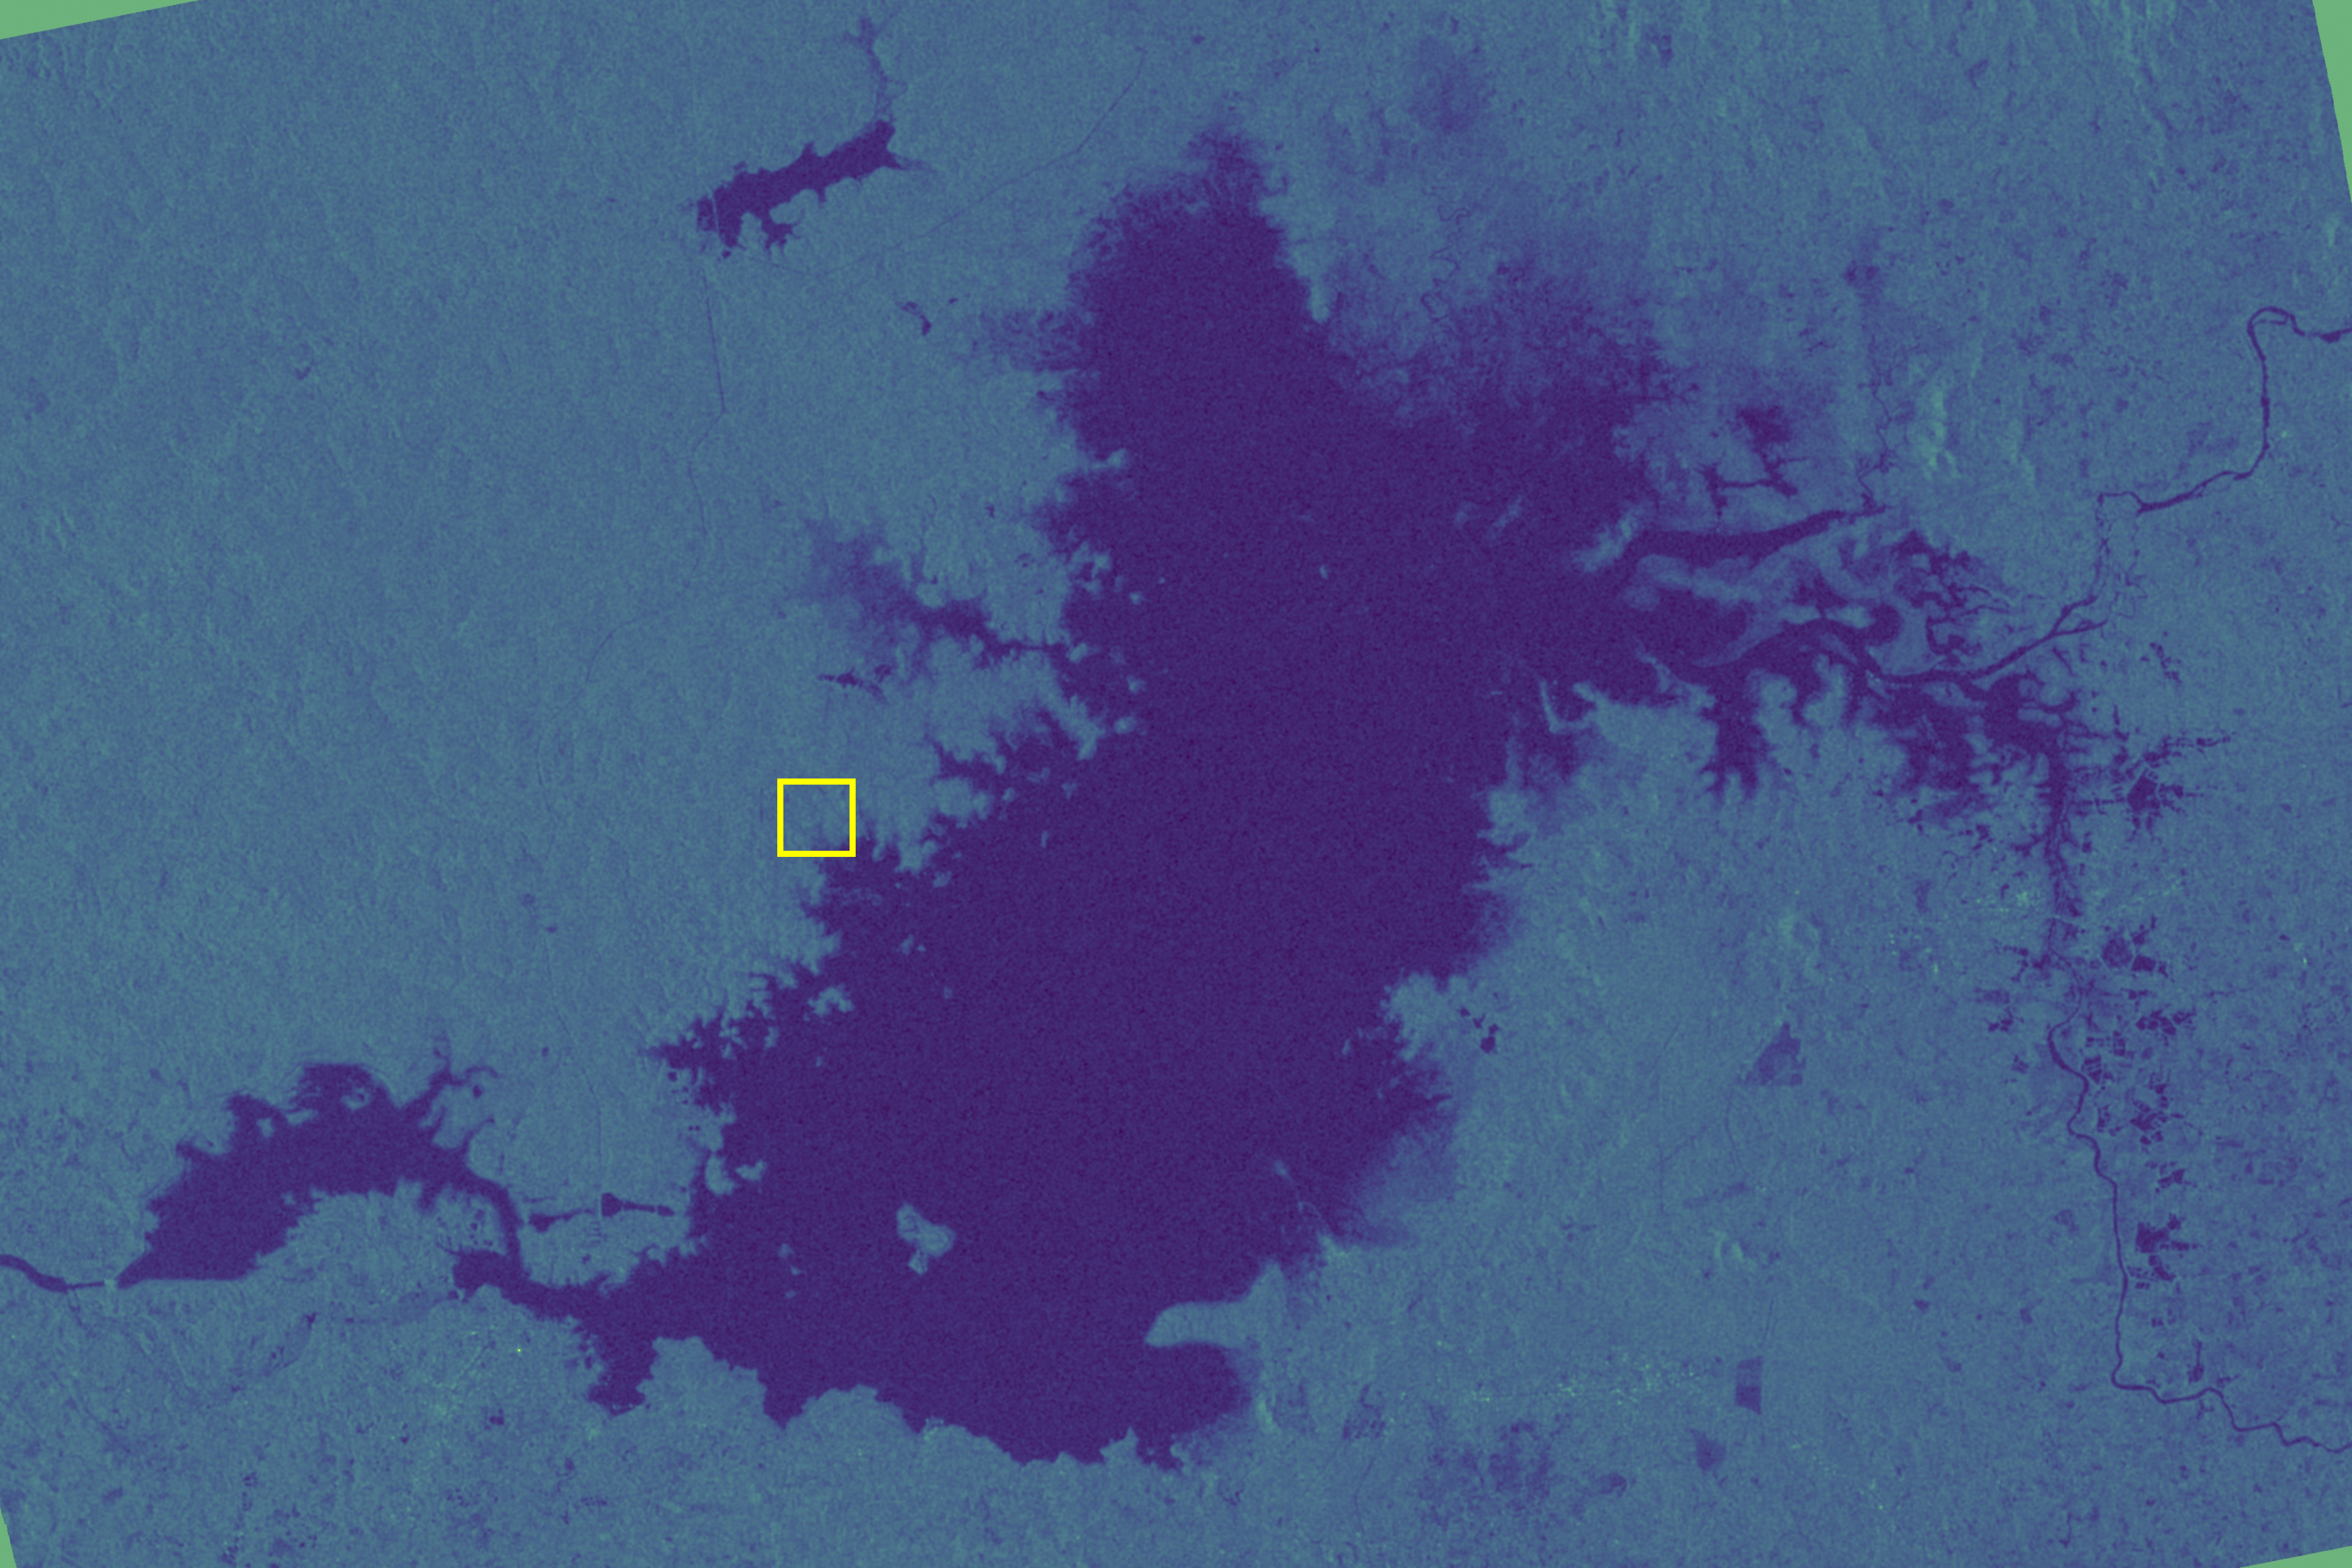
\includegraphics[width=0.3\linewidth]{figures/inputDemo_chap5/06.jpg}
        \end{tabular}
        \begin{tabular}[b]{c}
            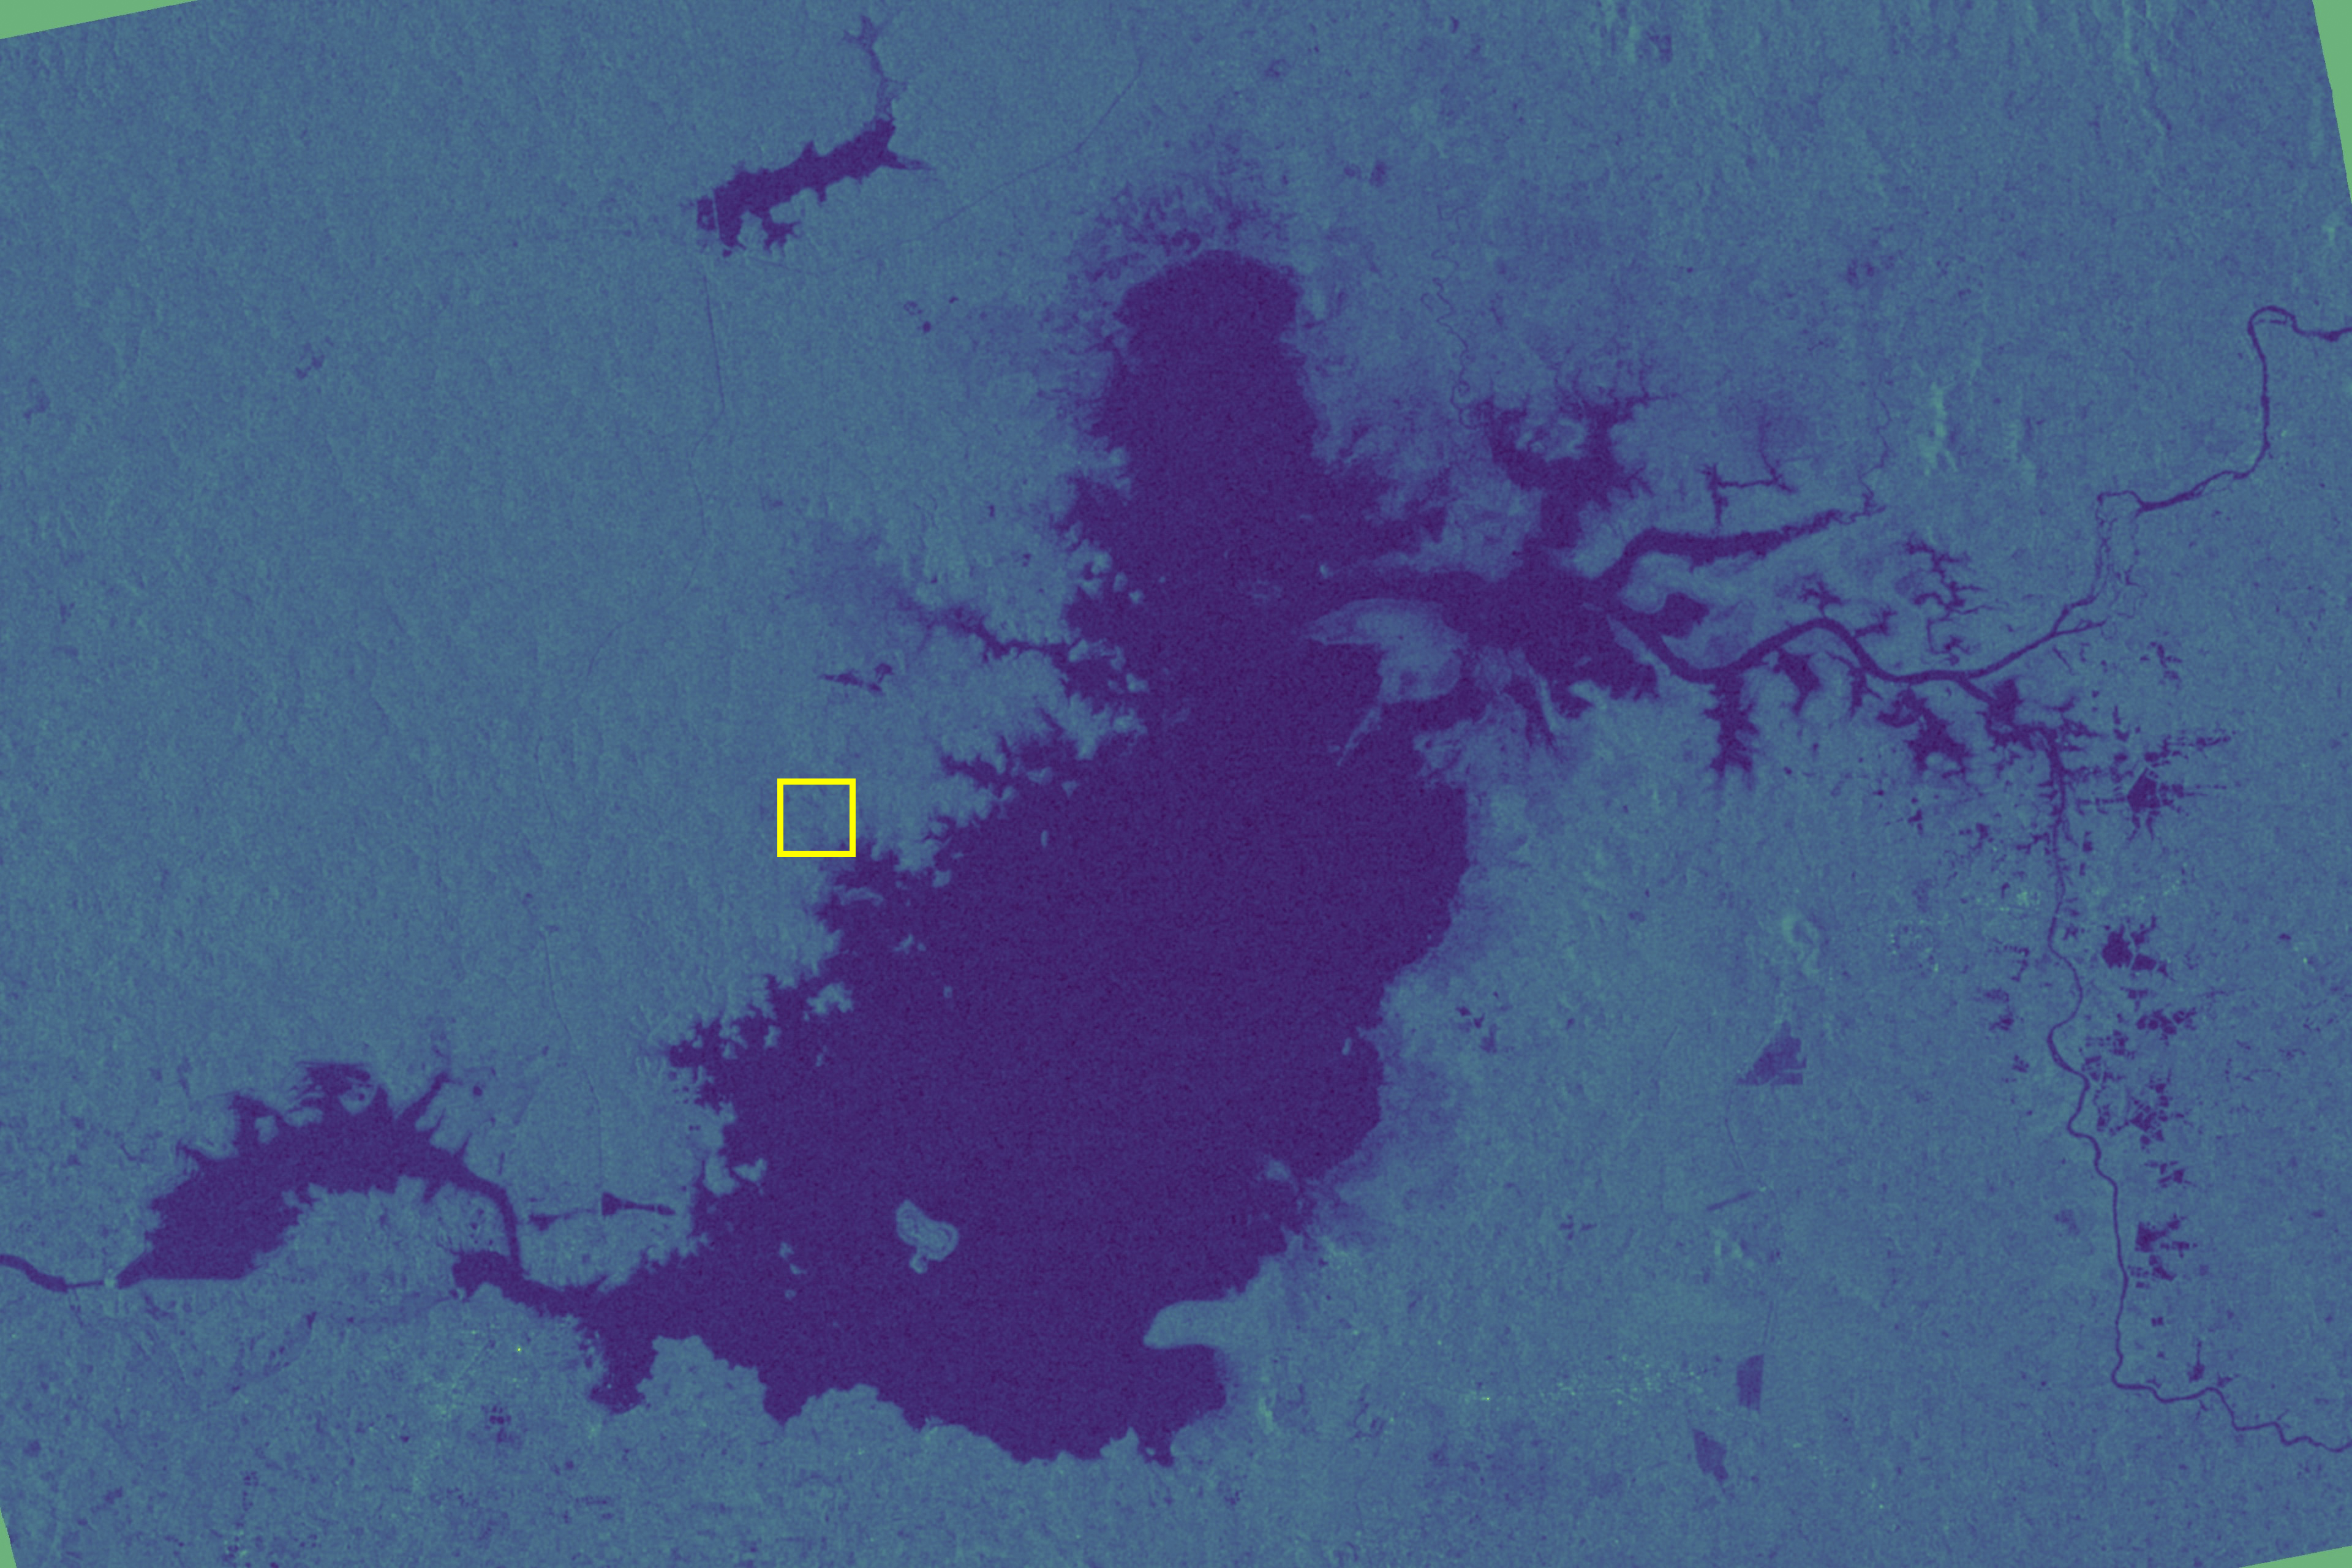
\includegraphics[width=0.3\linewidth]{figures/inputDemo_chap5/07.jpg}
        \end{tabular}
        \begin{tabular}[b]{c}
            \includegraphics[width=0.3\linewidth]{figures/inputDemo_chap5/08.jpg}
		\end{tabular}
        \begin{tabular}[b]{c}
            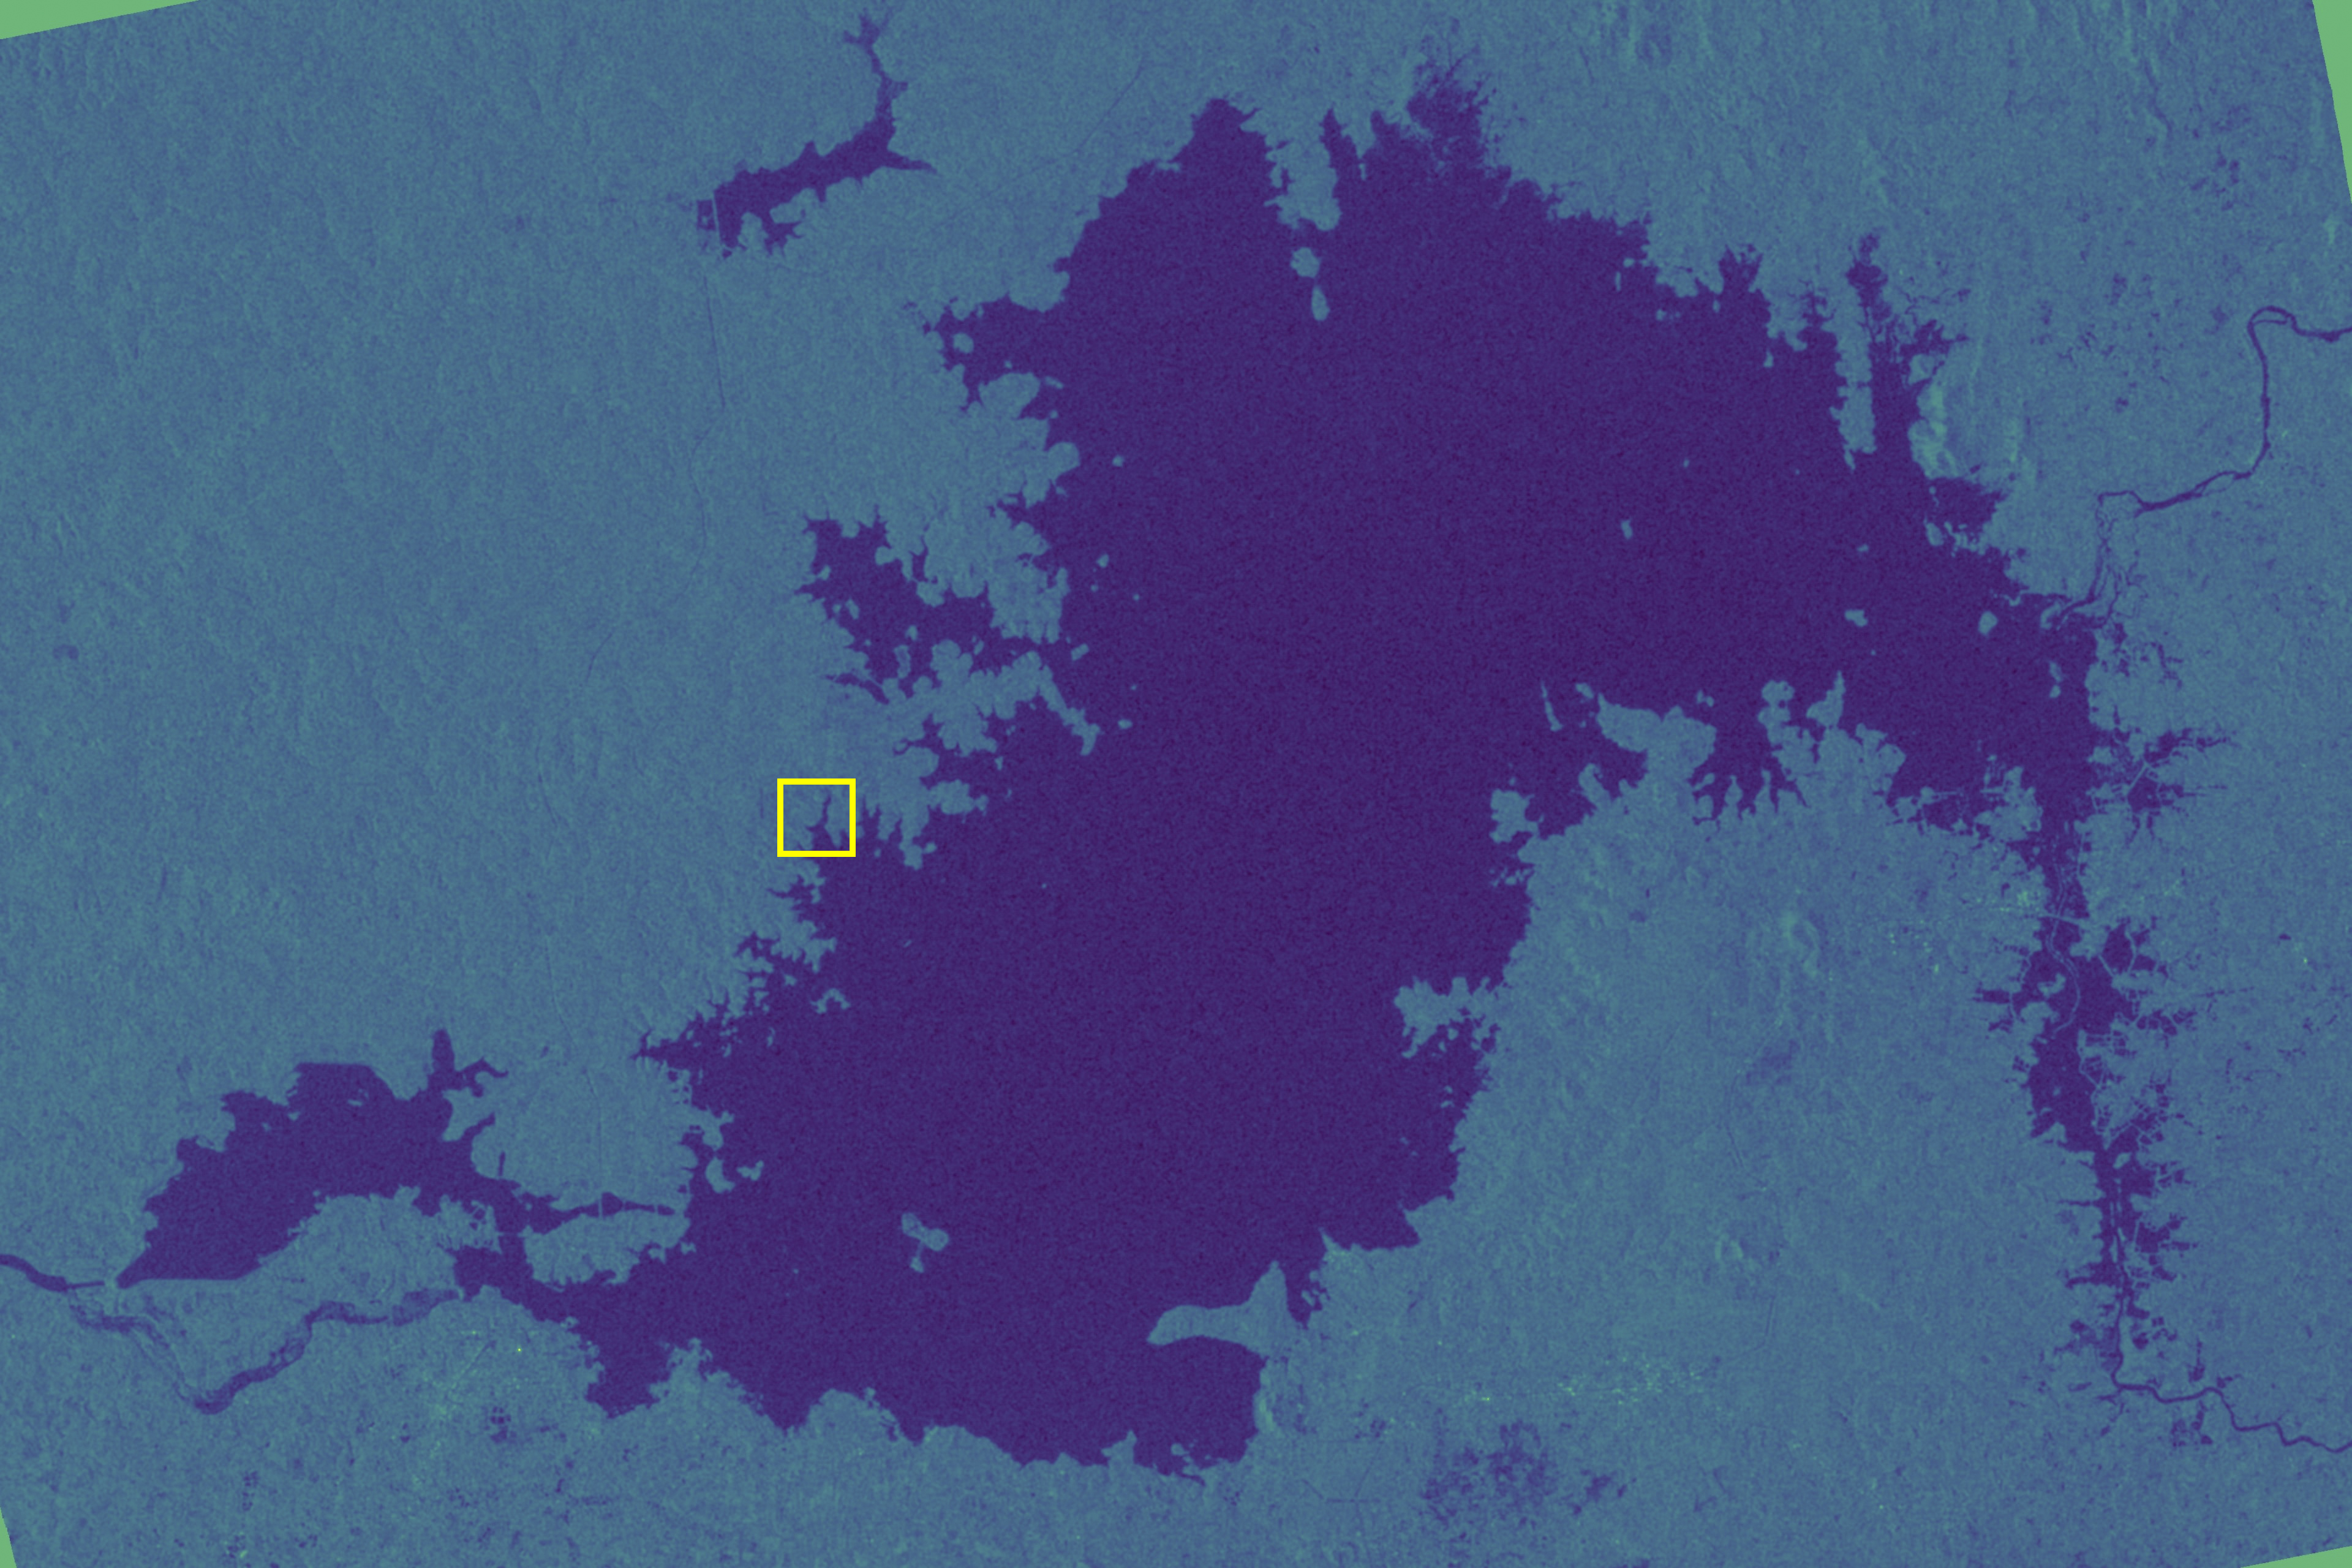
\includegraphics[width=0.3\linewidth]{figures/inputDemo_chap5/09.jpg}
        \end{tabular}
        \begin{tabular}[b]{c}
            \includegraphics[width=0.3\linewidth]{figures/inputDemo_chap5/10.jpg}
        \end{tabular}
        \begin{tabular}[b]{c}
            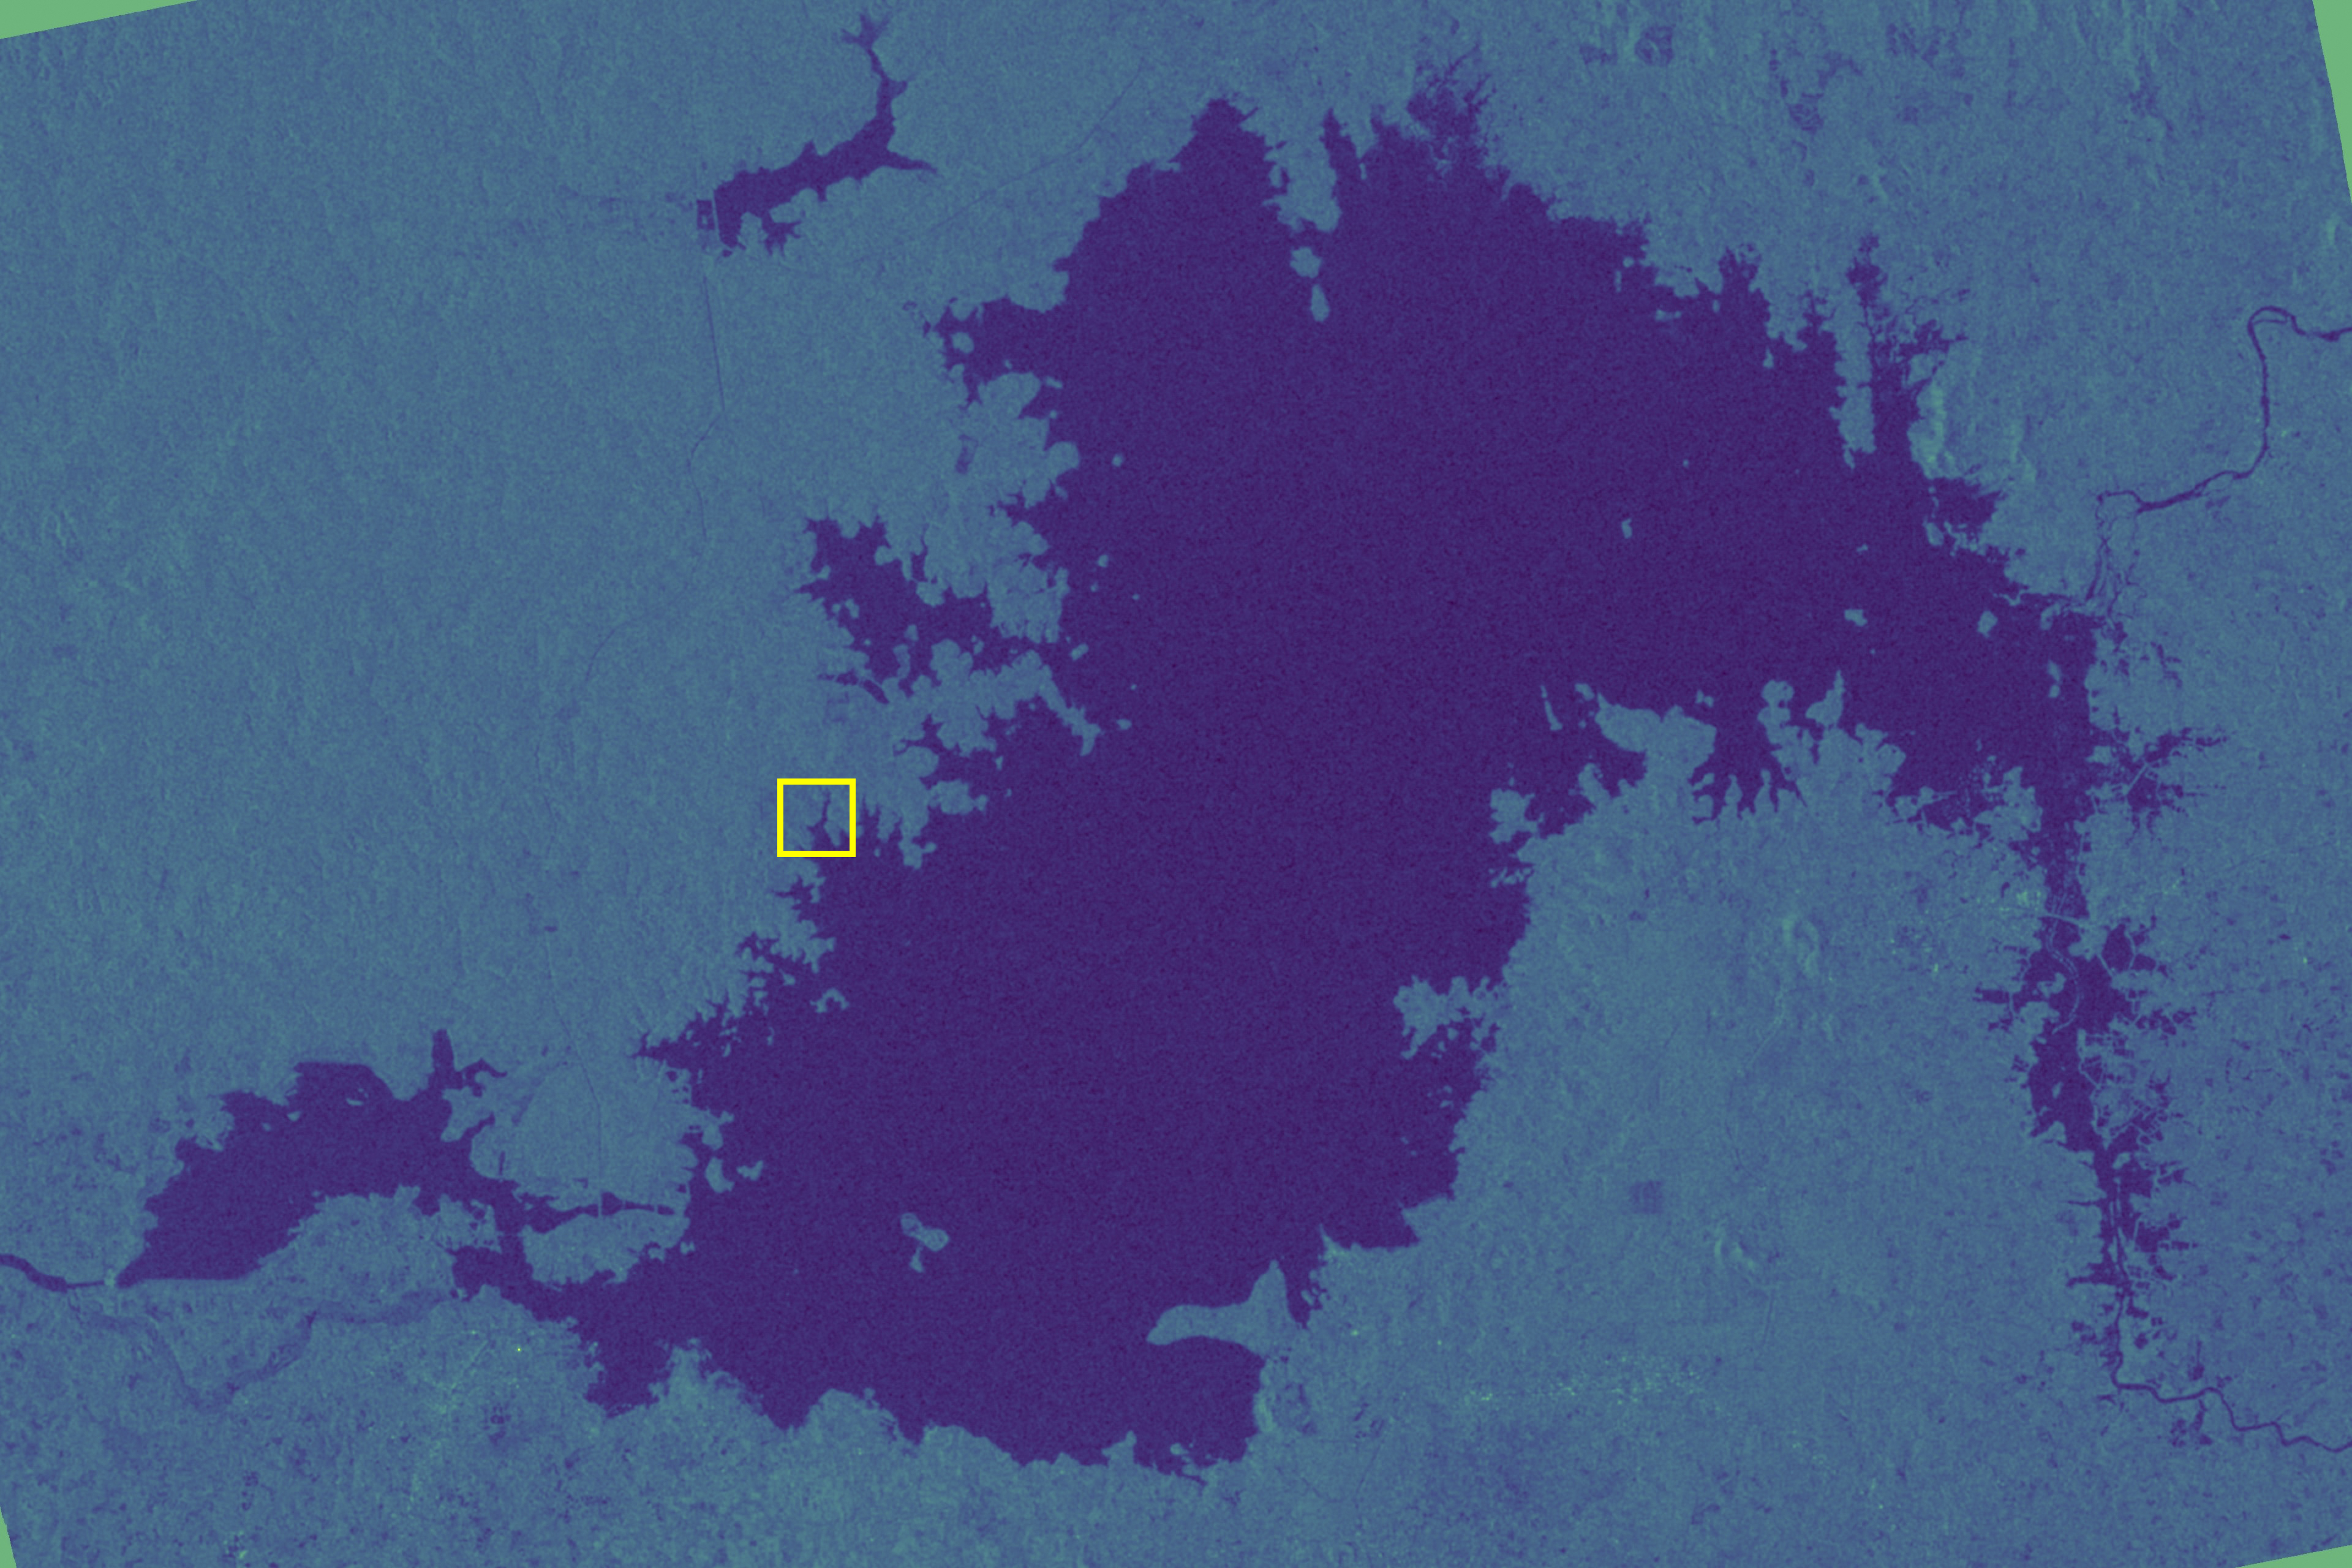
\includegraphics[width=0.3\linewidth]{figures/inputDemo_chap5/11.jpg}
		\end{tabular}
        \begin{tabular}[b]{c}
            \includegraphics[width=0.3\linewidth]{figures/inputDemo_chap5/12.jpg}
        \end{tabular}
        \begin{tabular}[b]{c}
            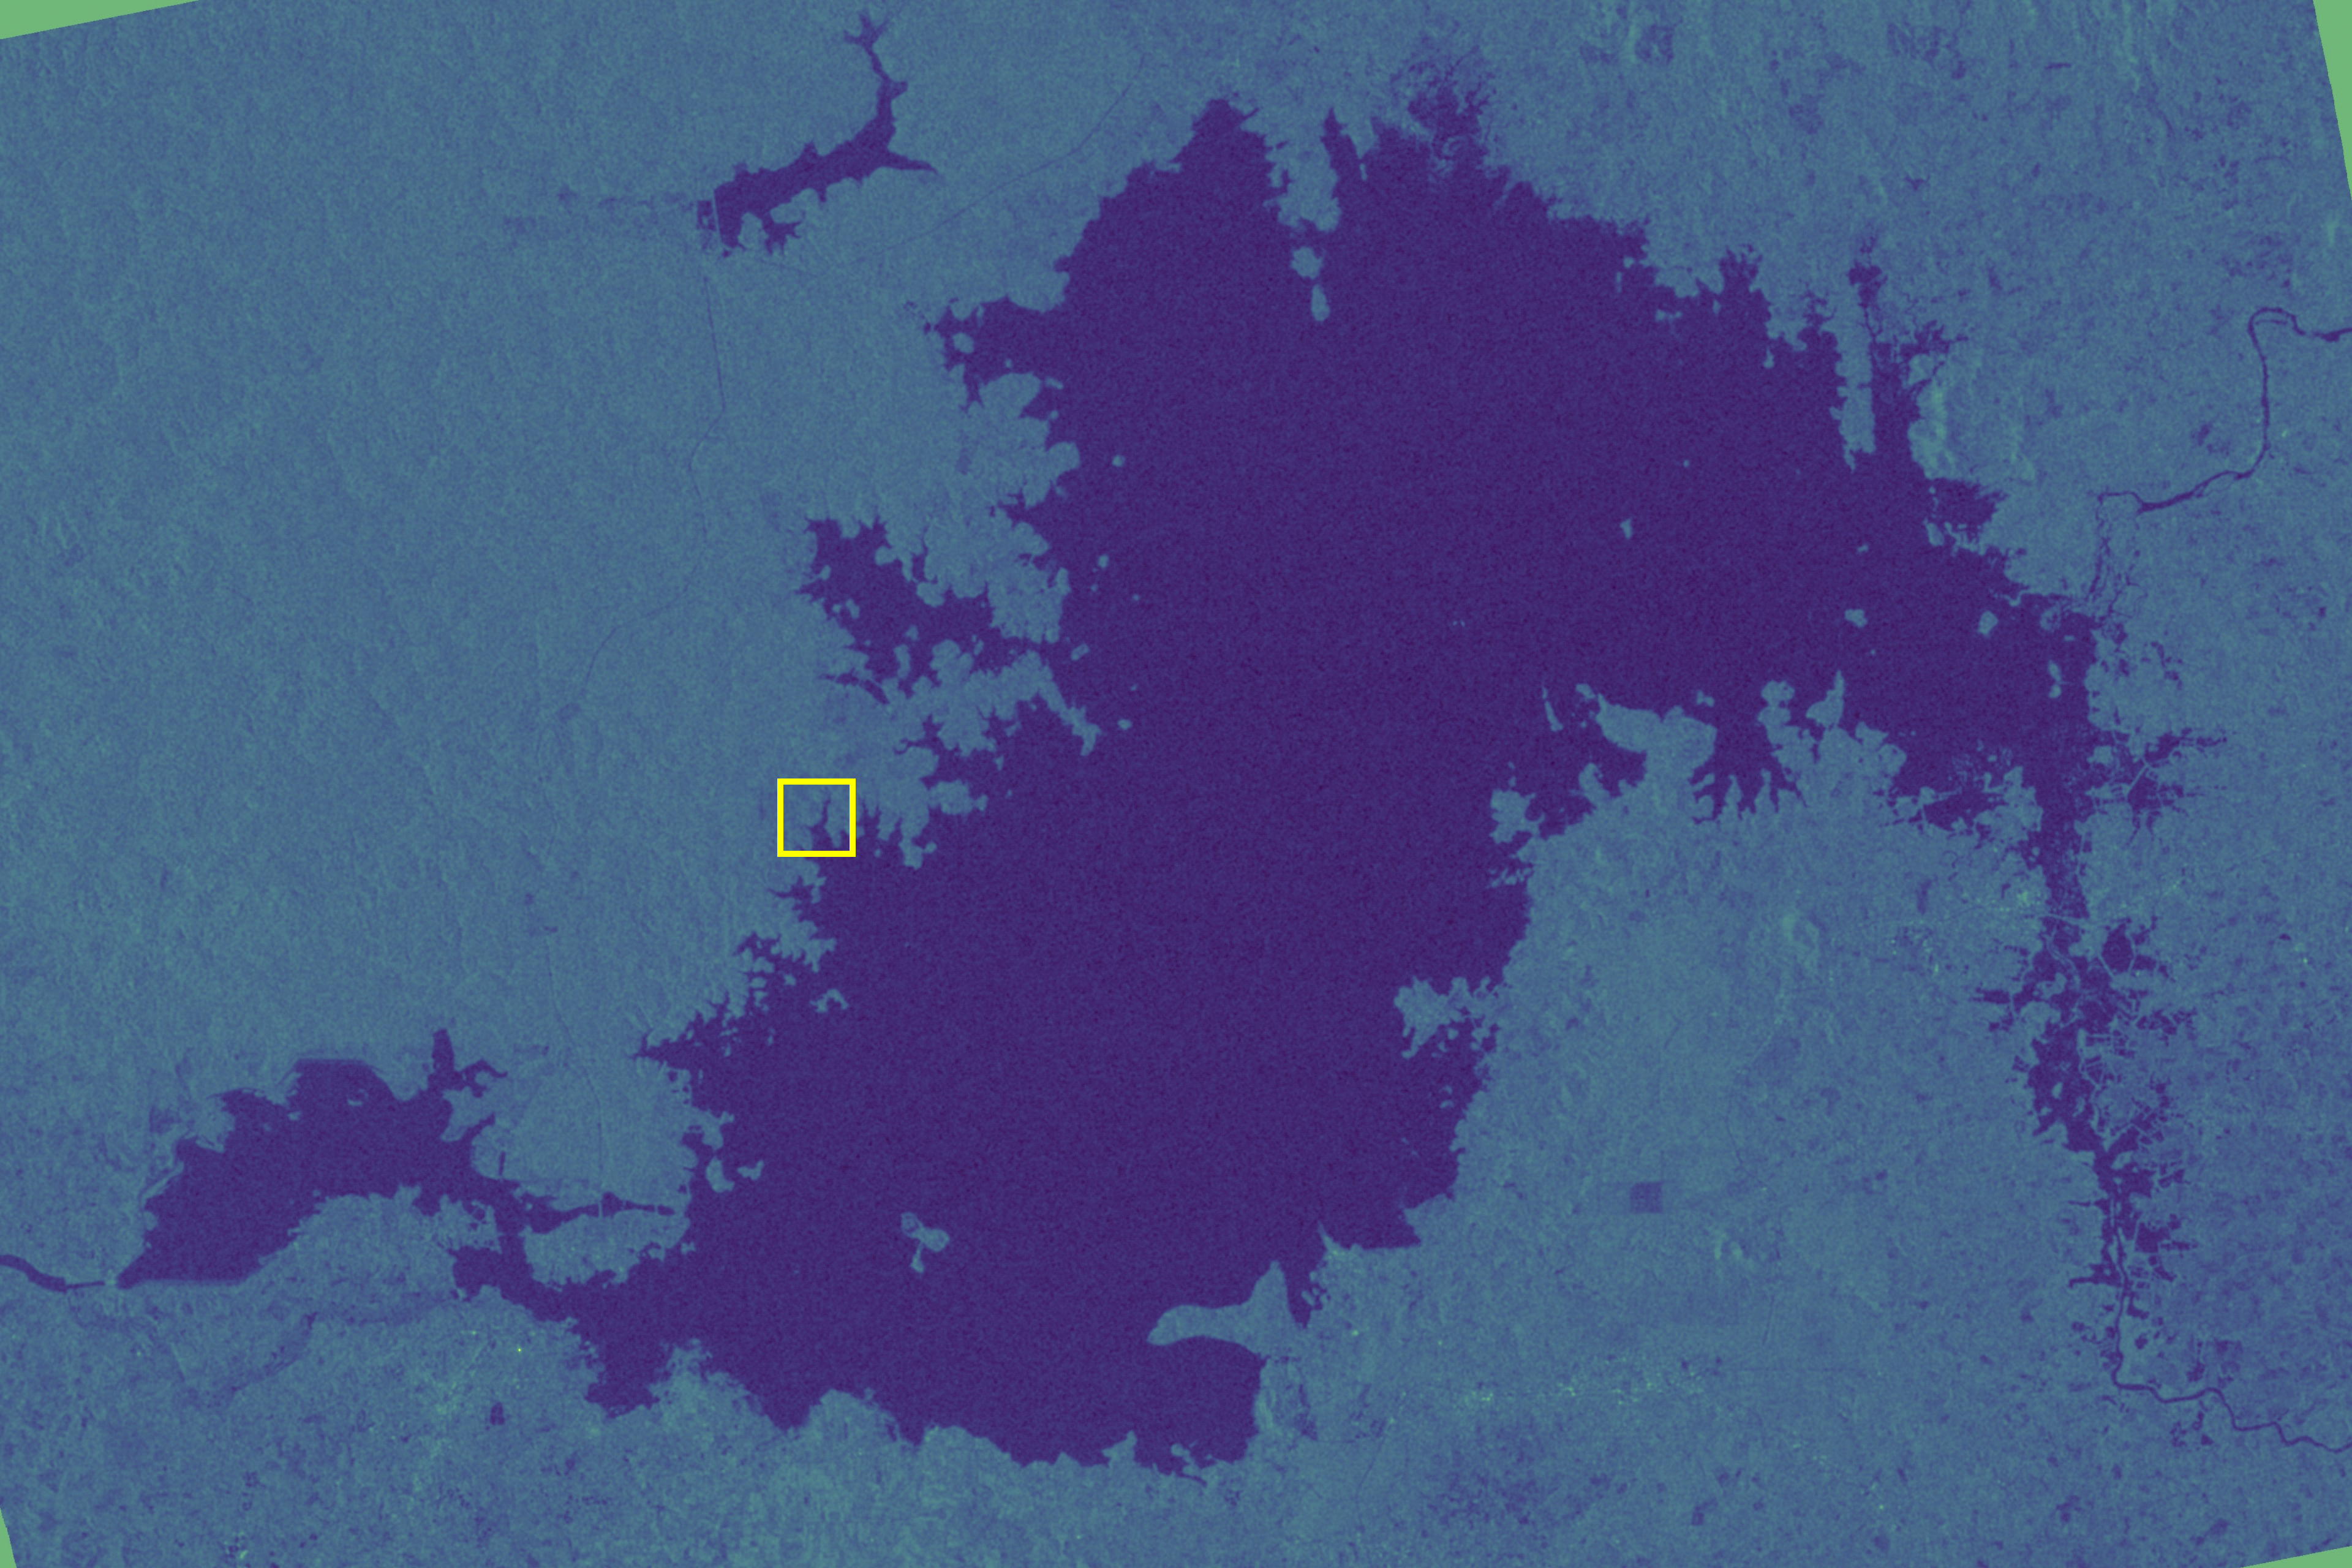
\includegraphics[width=0.3\linewidth]{figures/inputDemo_chap5/01.jpg}
        \end{tabular}
        \begin{tabular}[b]{c}
            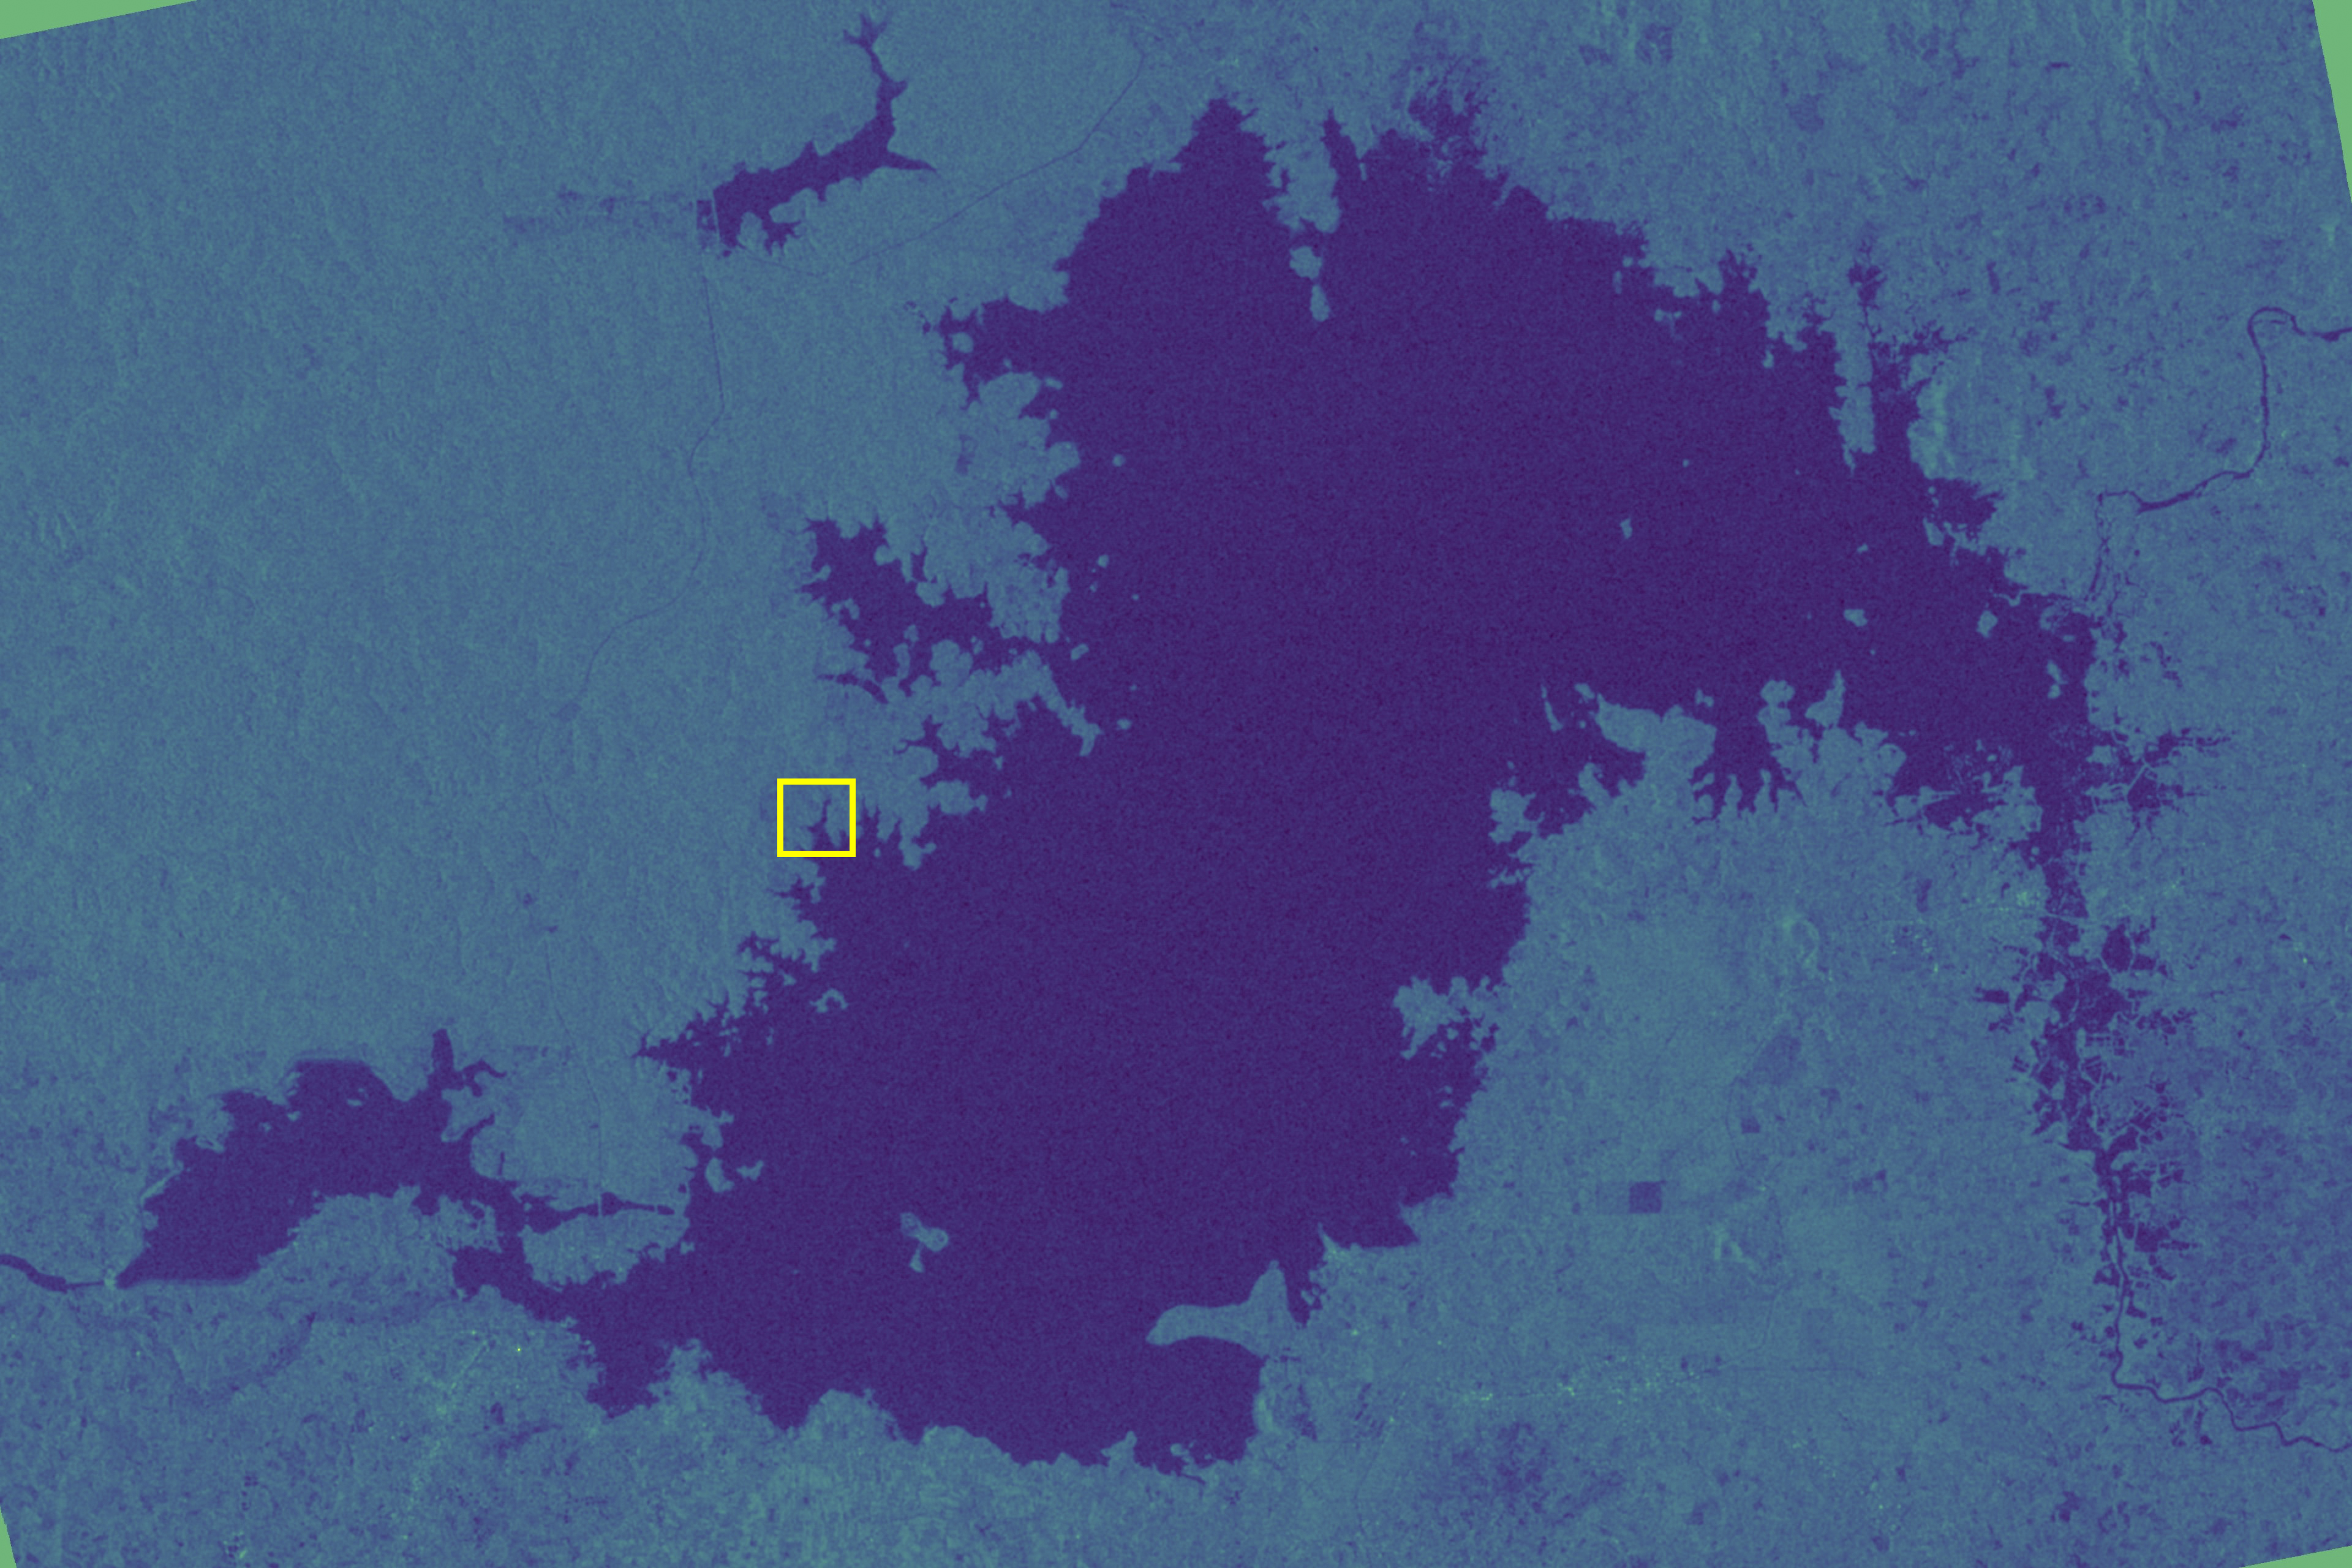
\includegraphics[width=0.3\linewidth]{figures/inputDemo_chap5/02.jpg}
		\end{tabular}
        \begin{tabular}[b]{c}
            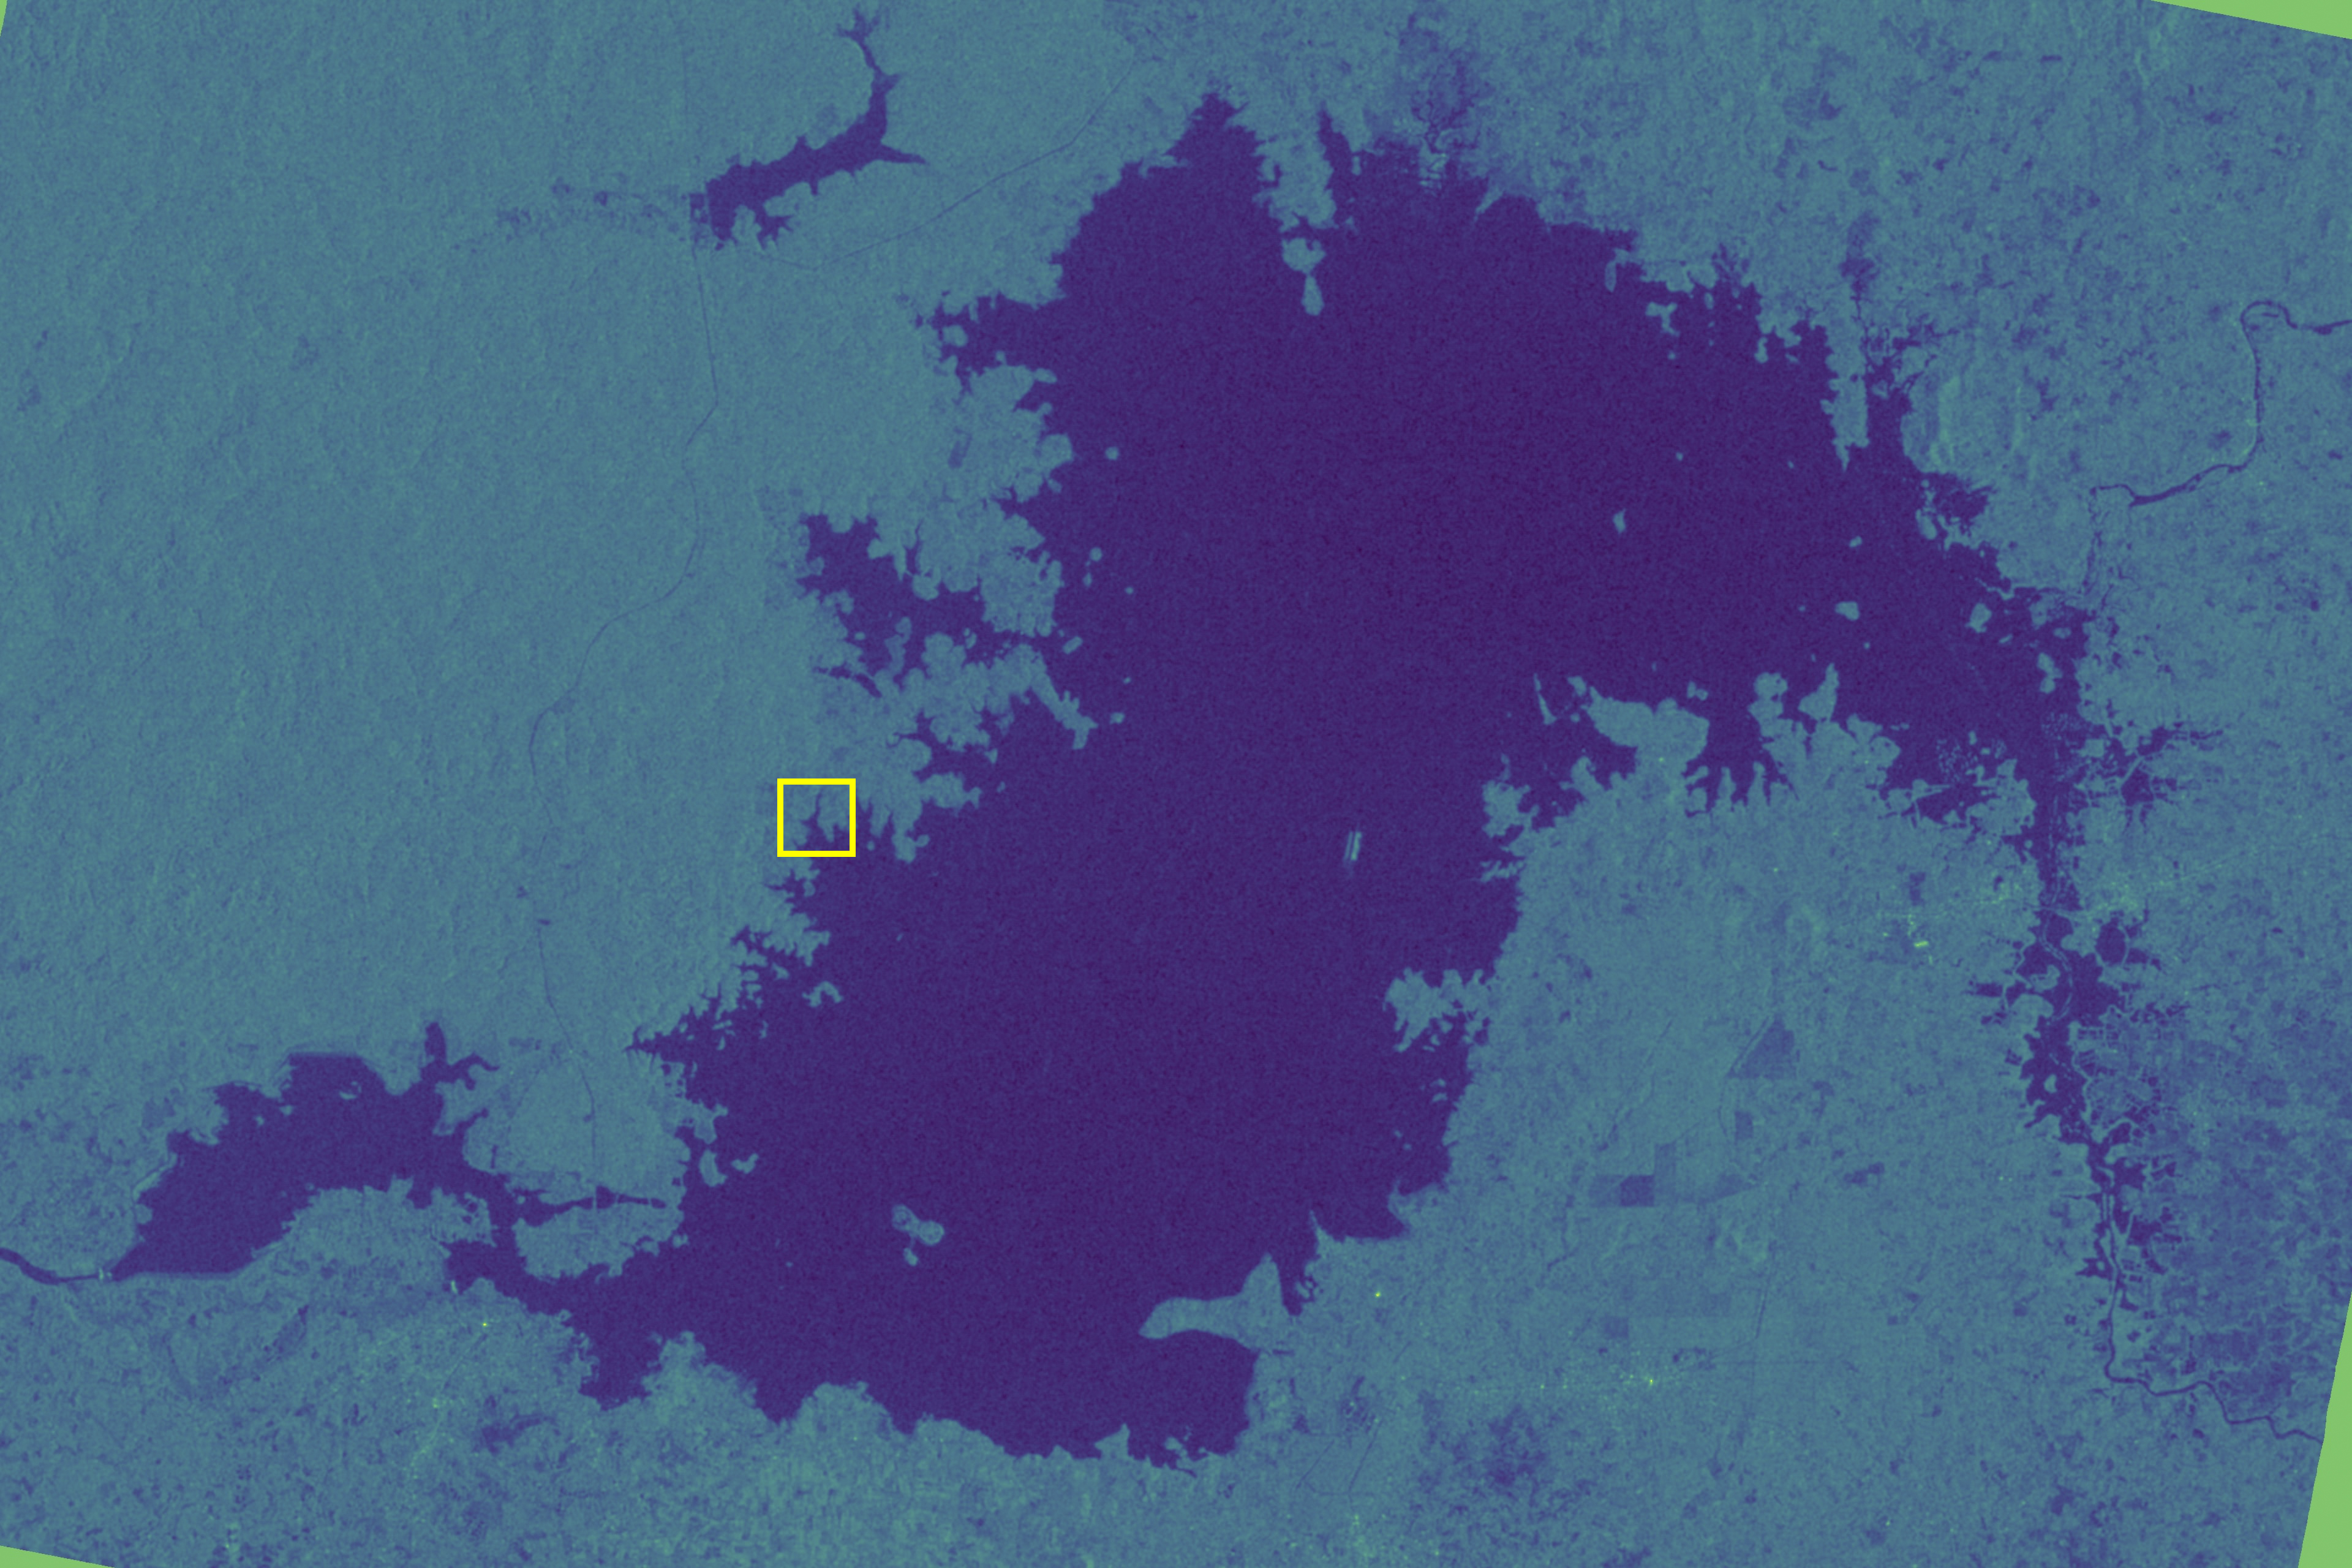
\includegraphics[width=0.3\linewidth]{figures/inputDemo_chap5/03.jpg}
        \end{tabular}
        \begin{tabular}[b]{c}
            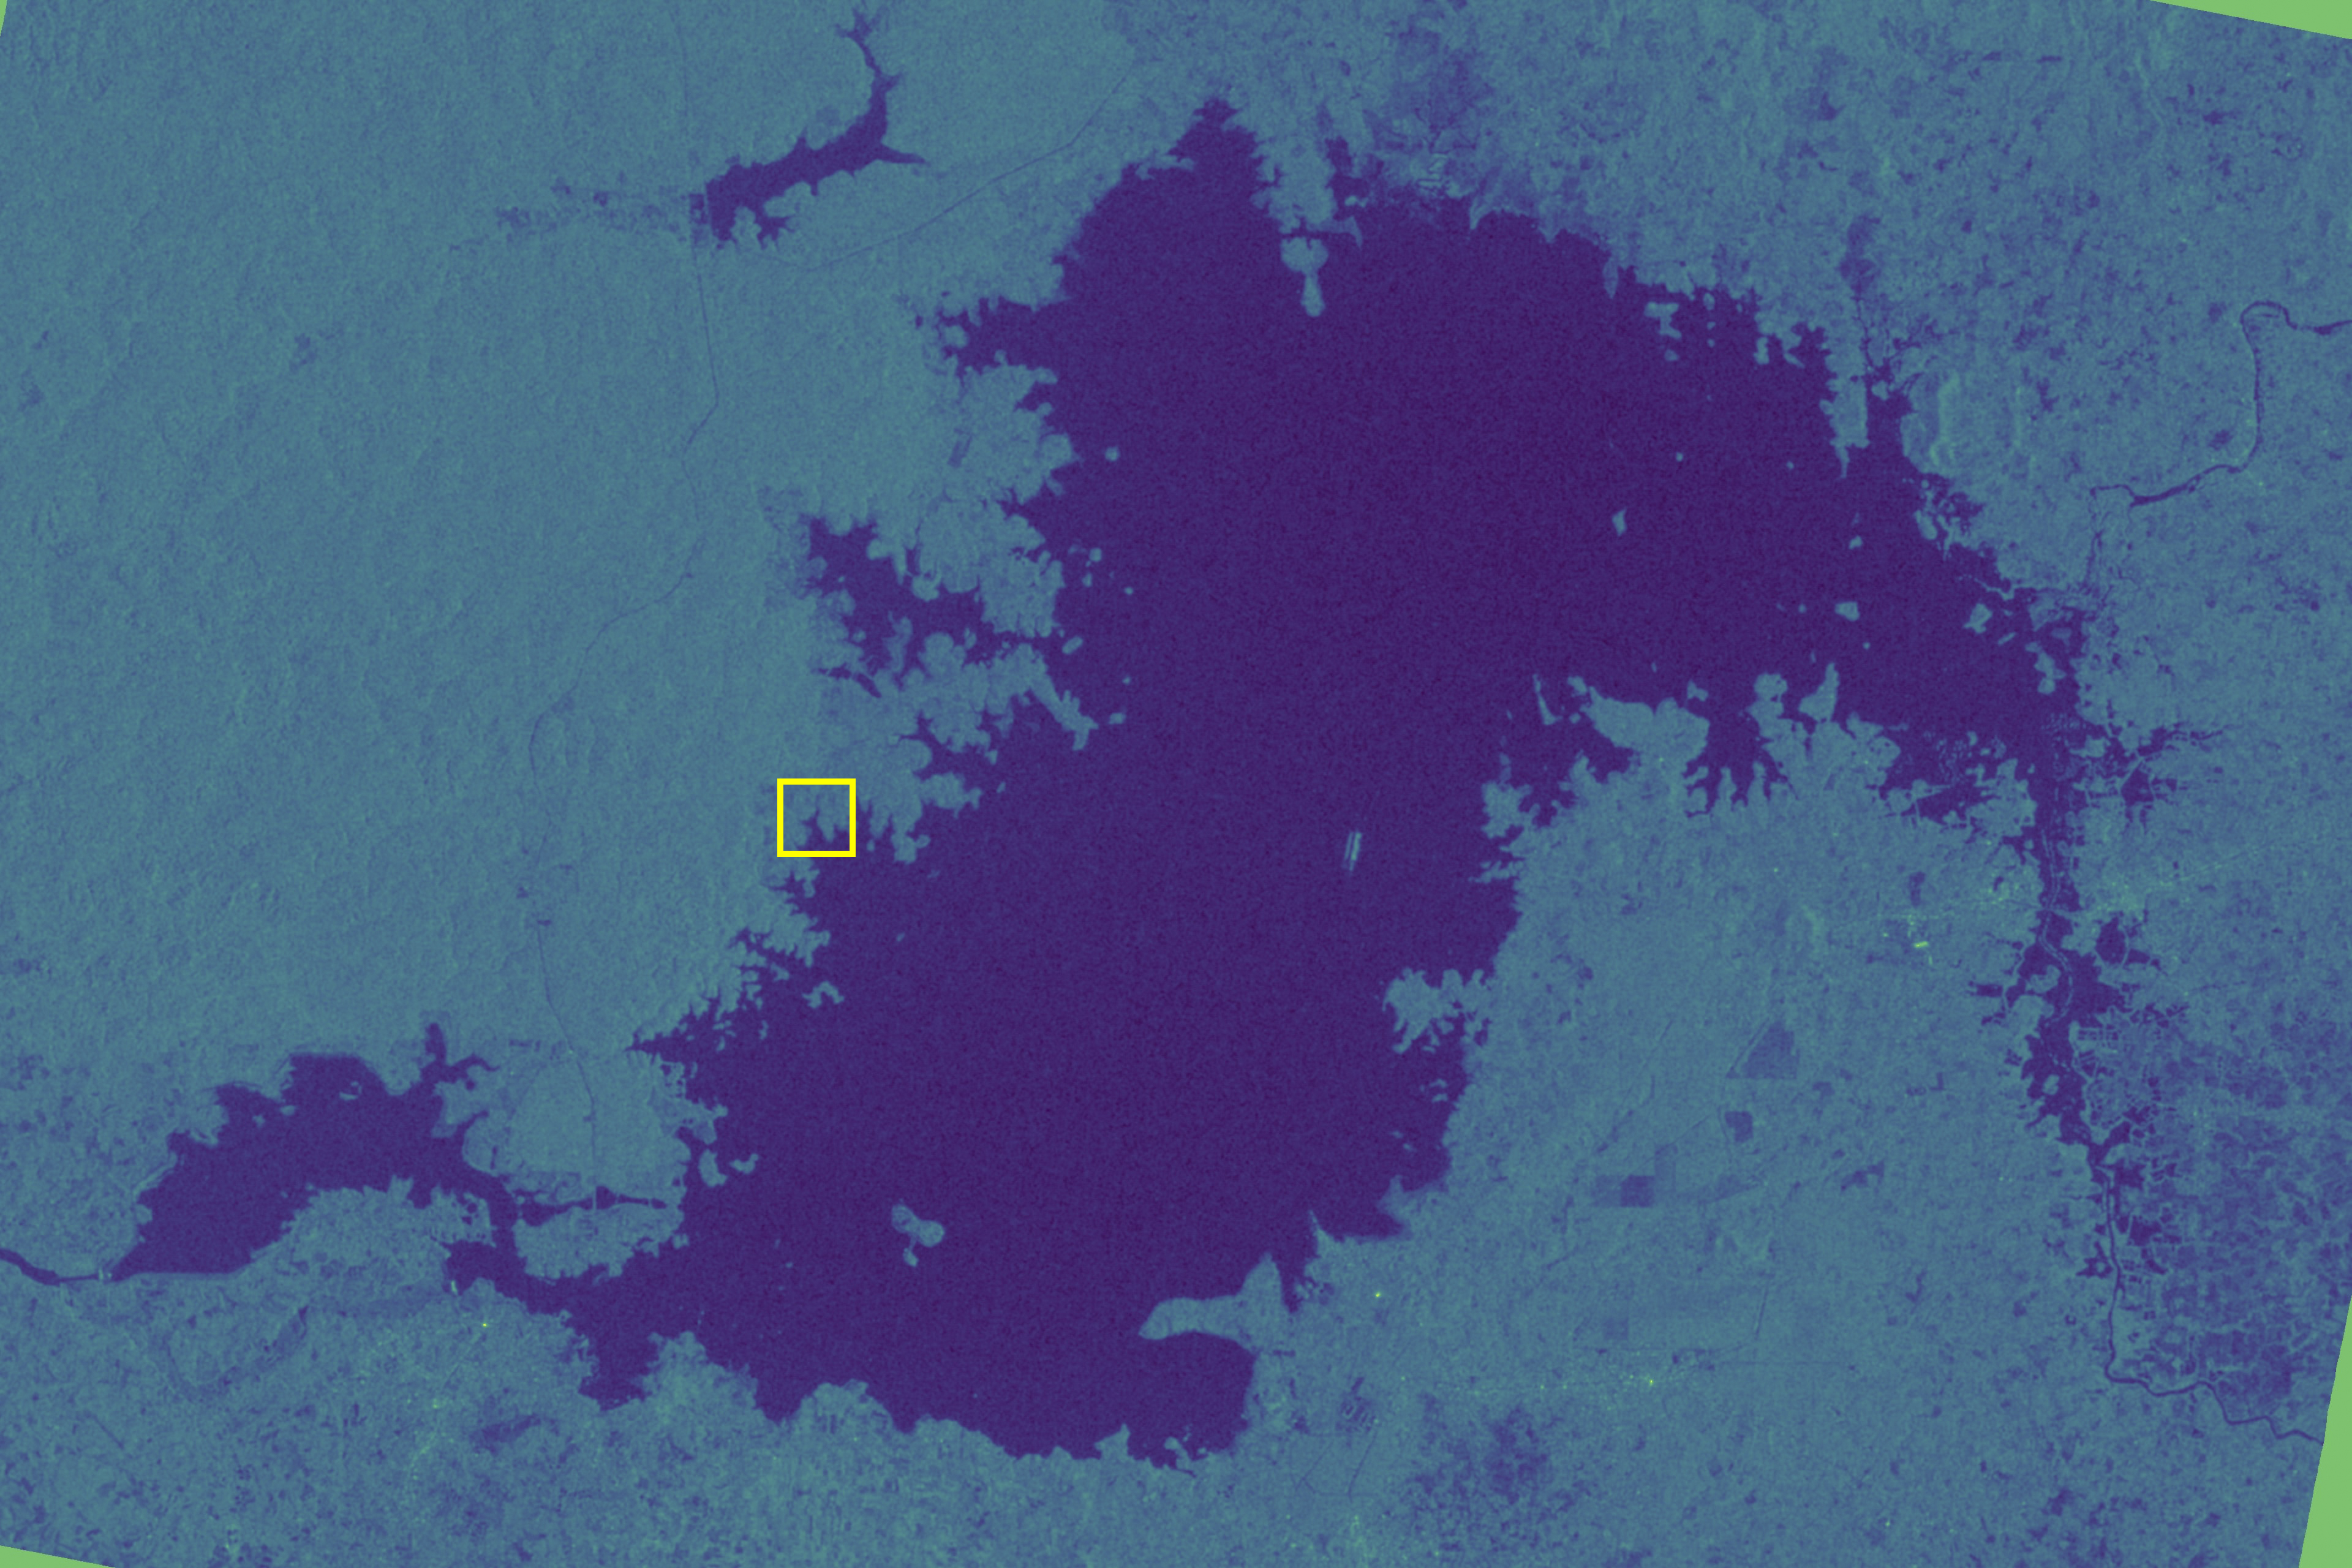
\includegraphics[width=0.3\linewidth]{figures/inputDemo_chap5/04.jpg}
        \end{tabular}
        \begin{tabular}[b]{c}
            \includegraphics[width=0.3\linewidth]{figures/inputDemo_chap5/05.jpg}
		\end{tabular} 
    \end{center}
	\caption[]{Sample input. From left to right, top to bottom: Time-series sequence from June 2018 to May 2019.}
	\label{fig:inputTs}
\end{figure}

\begin{figure}[h!]
	\centering
	\includegraphics[width=1\textwidth]{figures/tileInput.png}
	\caption[]{Input as tile to model, cropped from original in Figure \ref{fig:inputTs}}
	\label{fig:tileInputTs}
\end{figure}

The groundtruth output from above input is shown at Figure \ref{fig:outputTs}.

\begin{figure}[h!]
	\centering
	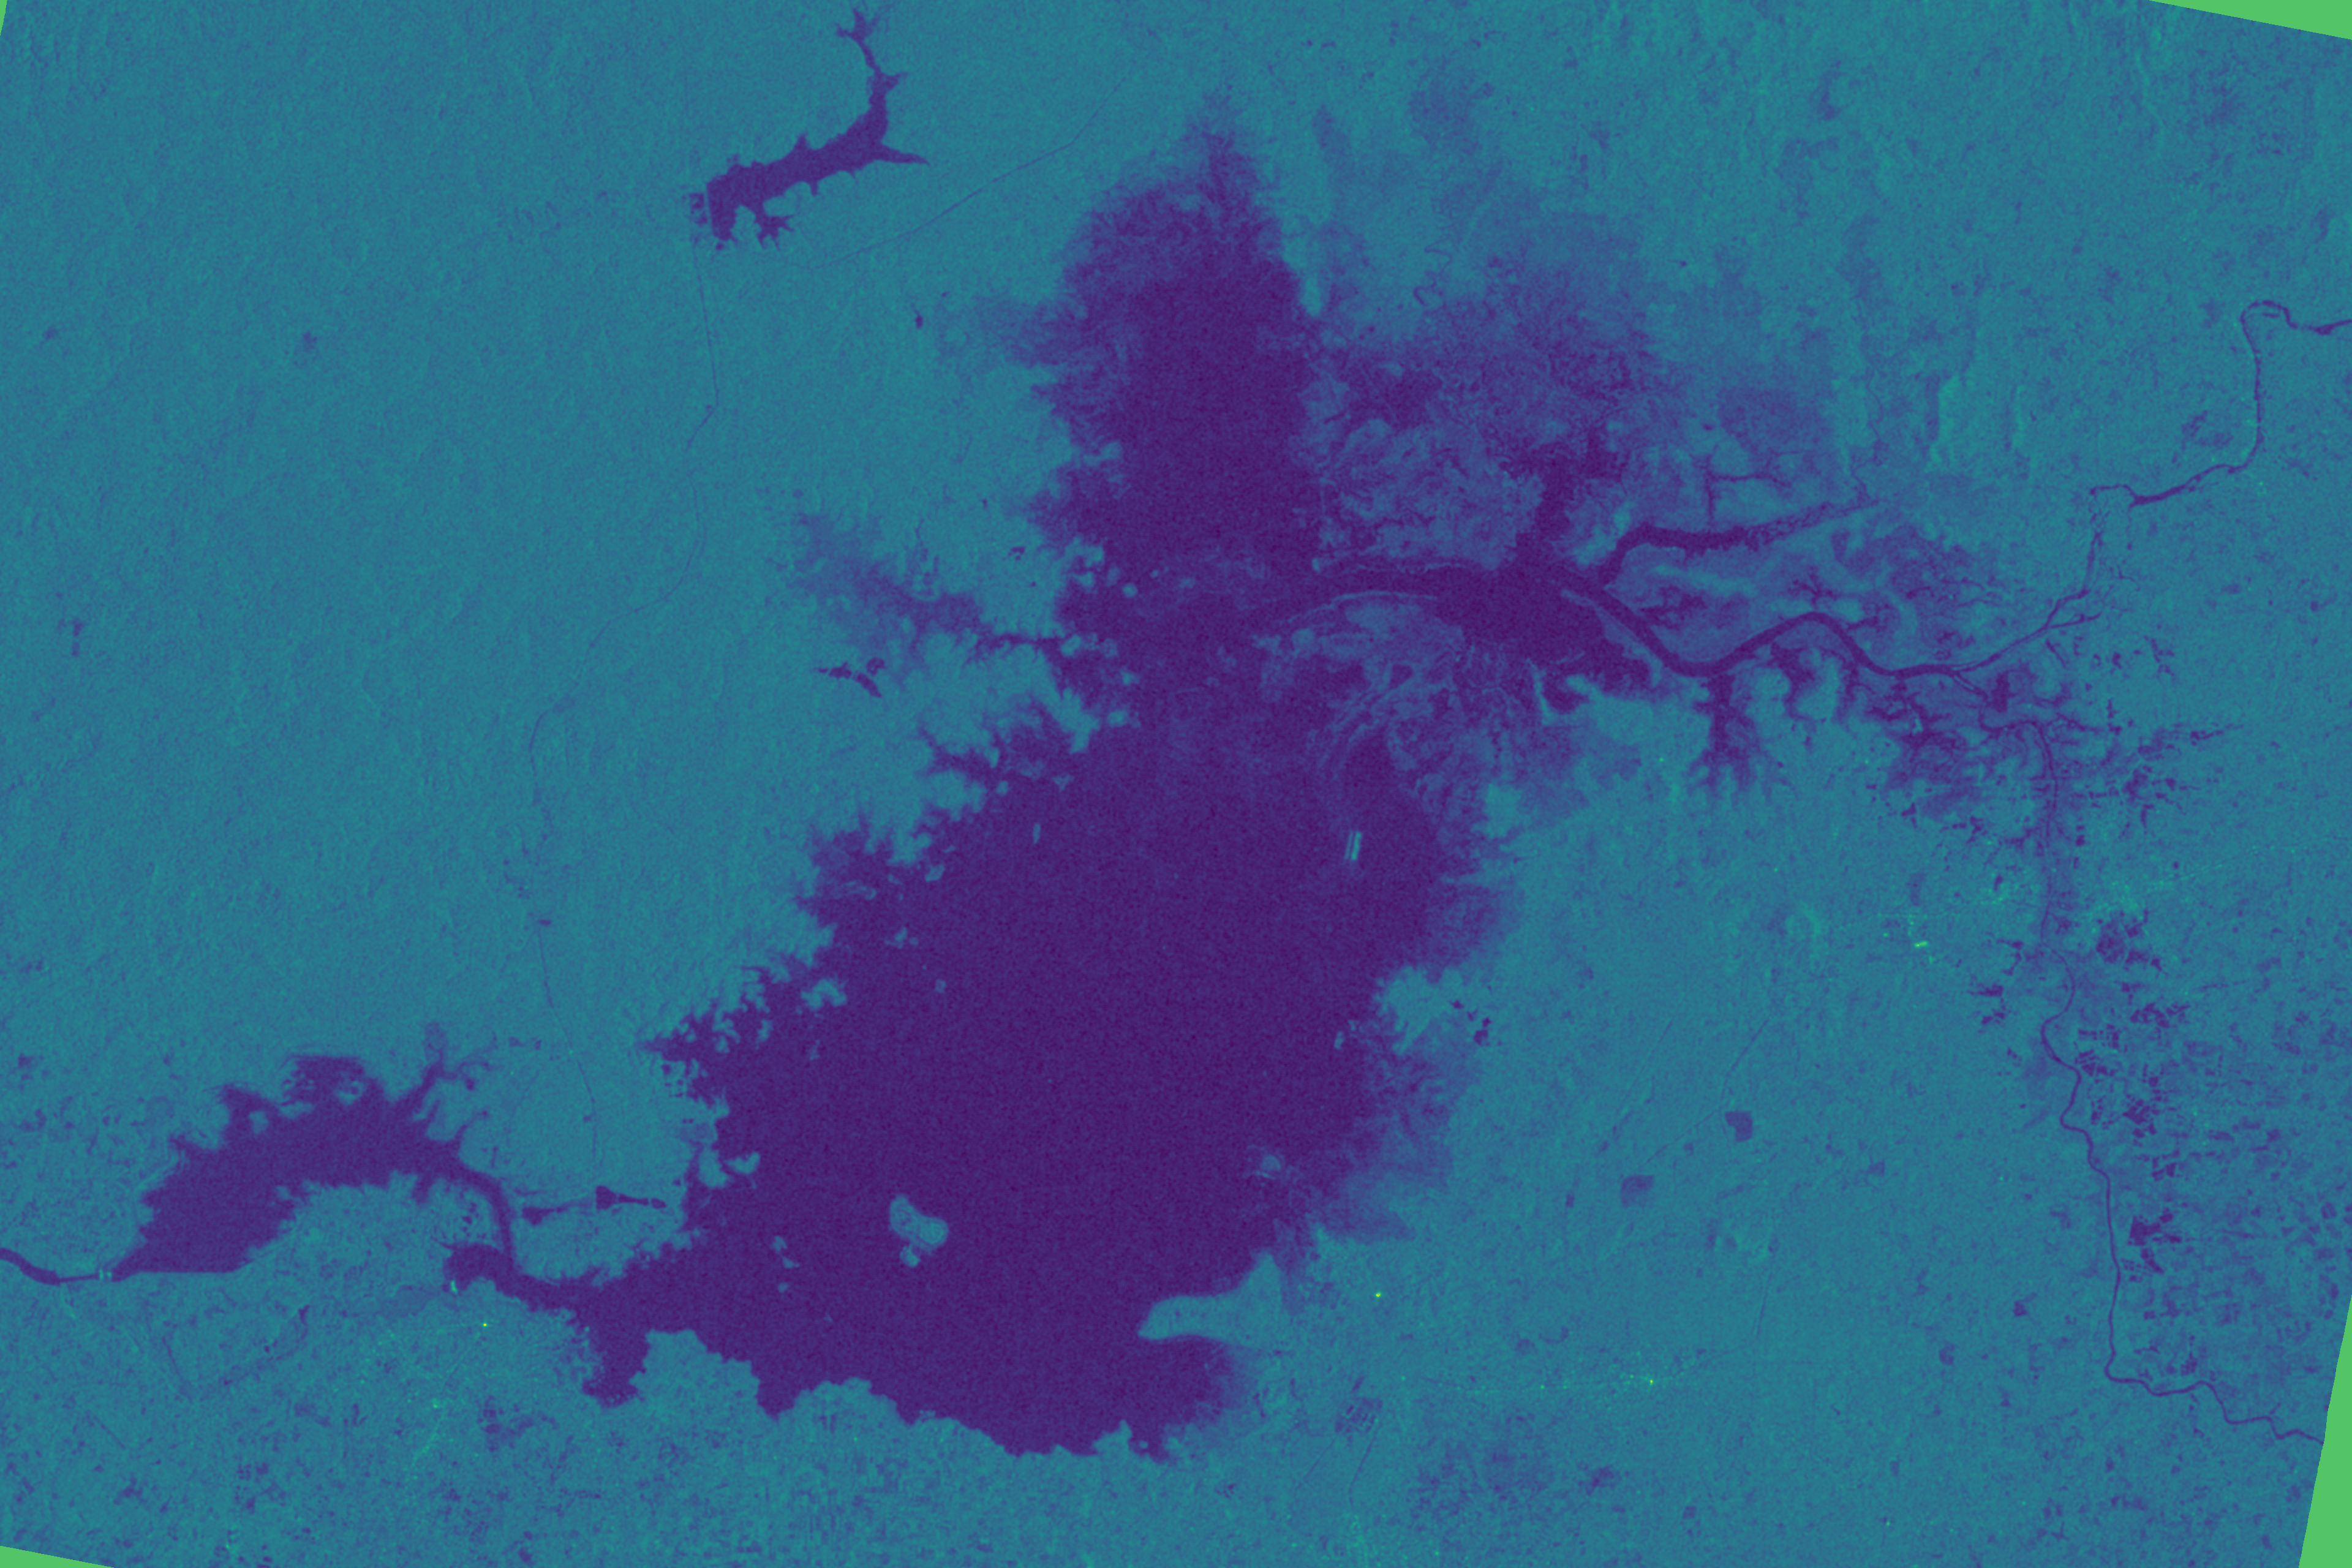
\includegraphics[width=1\textwidth]{figures/output_ts.png}
	\caption[]{Sample output: Groundtruth of water body in next time of sequence, June 2019.}
	\label{fig:outputTs}
\end{figure}

The prediction result of model, from Feb 2019 to June 2019 is shown in table \ref{table:predictValue}.

% Show table, contains result

\begin{table}[h!]
	\centering
	\begin{tabularx}{\textwidth}{|Y|Y|Y|Y|Y|}
		\hline
		\textbf{Month} & \textbf{Groundtruth Area ($km^2$)} & \textbf{Predicted Area ($km^2$)} & \textbf{True Prediction Ratio (\%)} & \textbf{False Prediction Ratio (\%)}\\ \hline
		2              & 282.5946                                          & 287.7469                                        & 98.32 & 3.44                         \\ \hline
		3              & 296.5101                                          & 301.0503                                        & 97.02 & 
		4.44                          \\ \hline
		4              & 301.2402                                          & 276.8264                                        & 87.60 & 4.68                         \\ \hline
		5              & 273.7712                                          & 273.0462                                        & 96.39 & 3.35                          \\ \hline
		6              & 243.2829                                          & 217.7548                                        & 86.40 & 3.47                         \\ \hline
	\end{tabularx}
	\caption[]{Area prediction result and ratio}
	\label{table:predictValue}
\end{table}

% Plot predicted result, with groundtruth value

\begin{figure}[h!]
	\centering
	\includegraphics[width=1\textwidth]{figures/comparePredict.png}
	\caption[]{Area comparison between groundtruth and prediction.}
	\label{fig:comparePredict}
\end{figure}

Figure \ref{fig:prediction_02}, \ref{fig:prediction_03}, \ref{fig:prediction_04}, \ref{fig:prediction_05} and \ref{fig:prediction_06} are groundtruth and corresponding prediction for Tri An Reservoir water body from 12 previous months, from February to June 2019, in which the yellow line shows boundaries of predicted water body.

% Show 2-6/19 prediction, with result and boundaries.
\begin{figure}[h!]
	\centering
	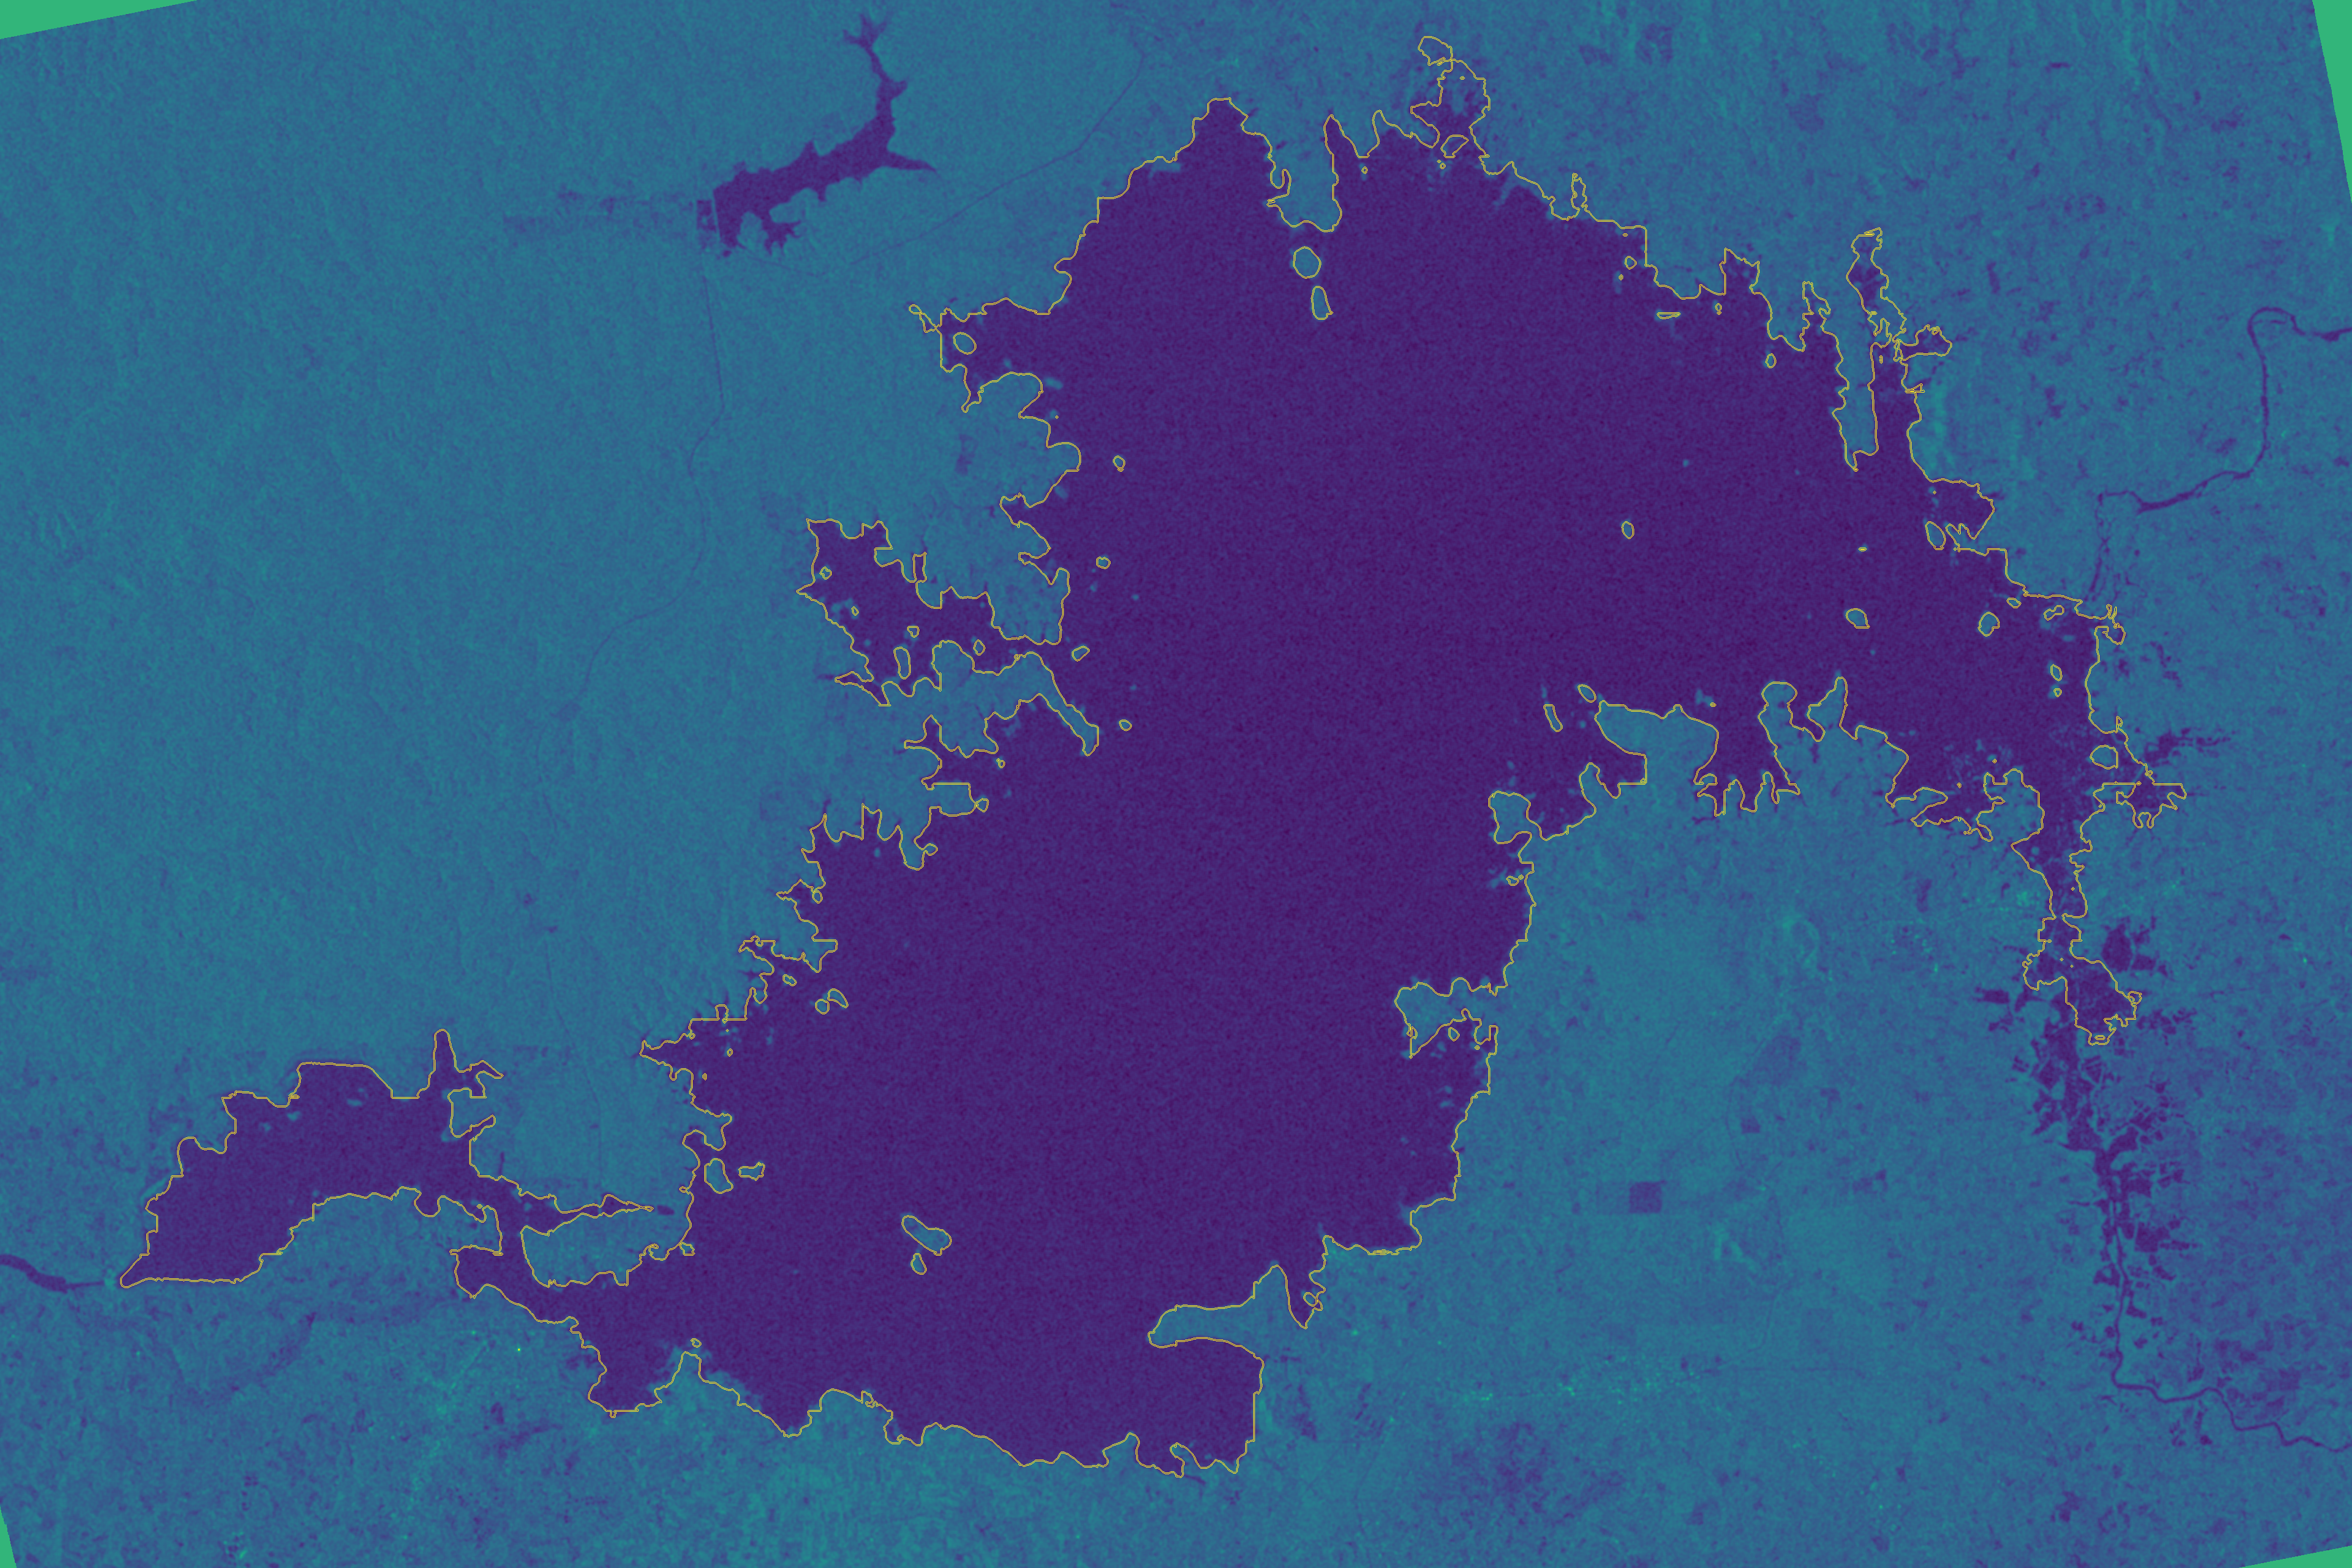
\includegraphics[width=0.9\textwidth]{figures/20190202T110307.png}
	\caption[]{Prediction, Feb 2019}
	\label{fig:prediction_02}
\end{figure}

\begin{figure}[h!]
	\centering
	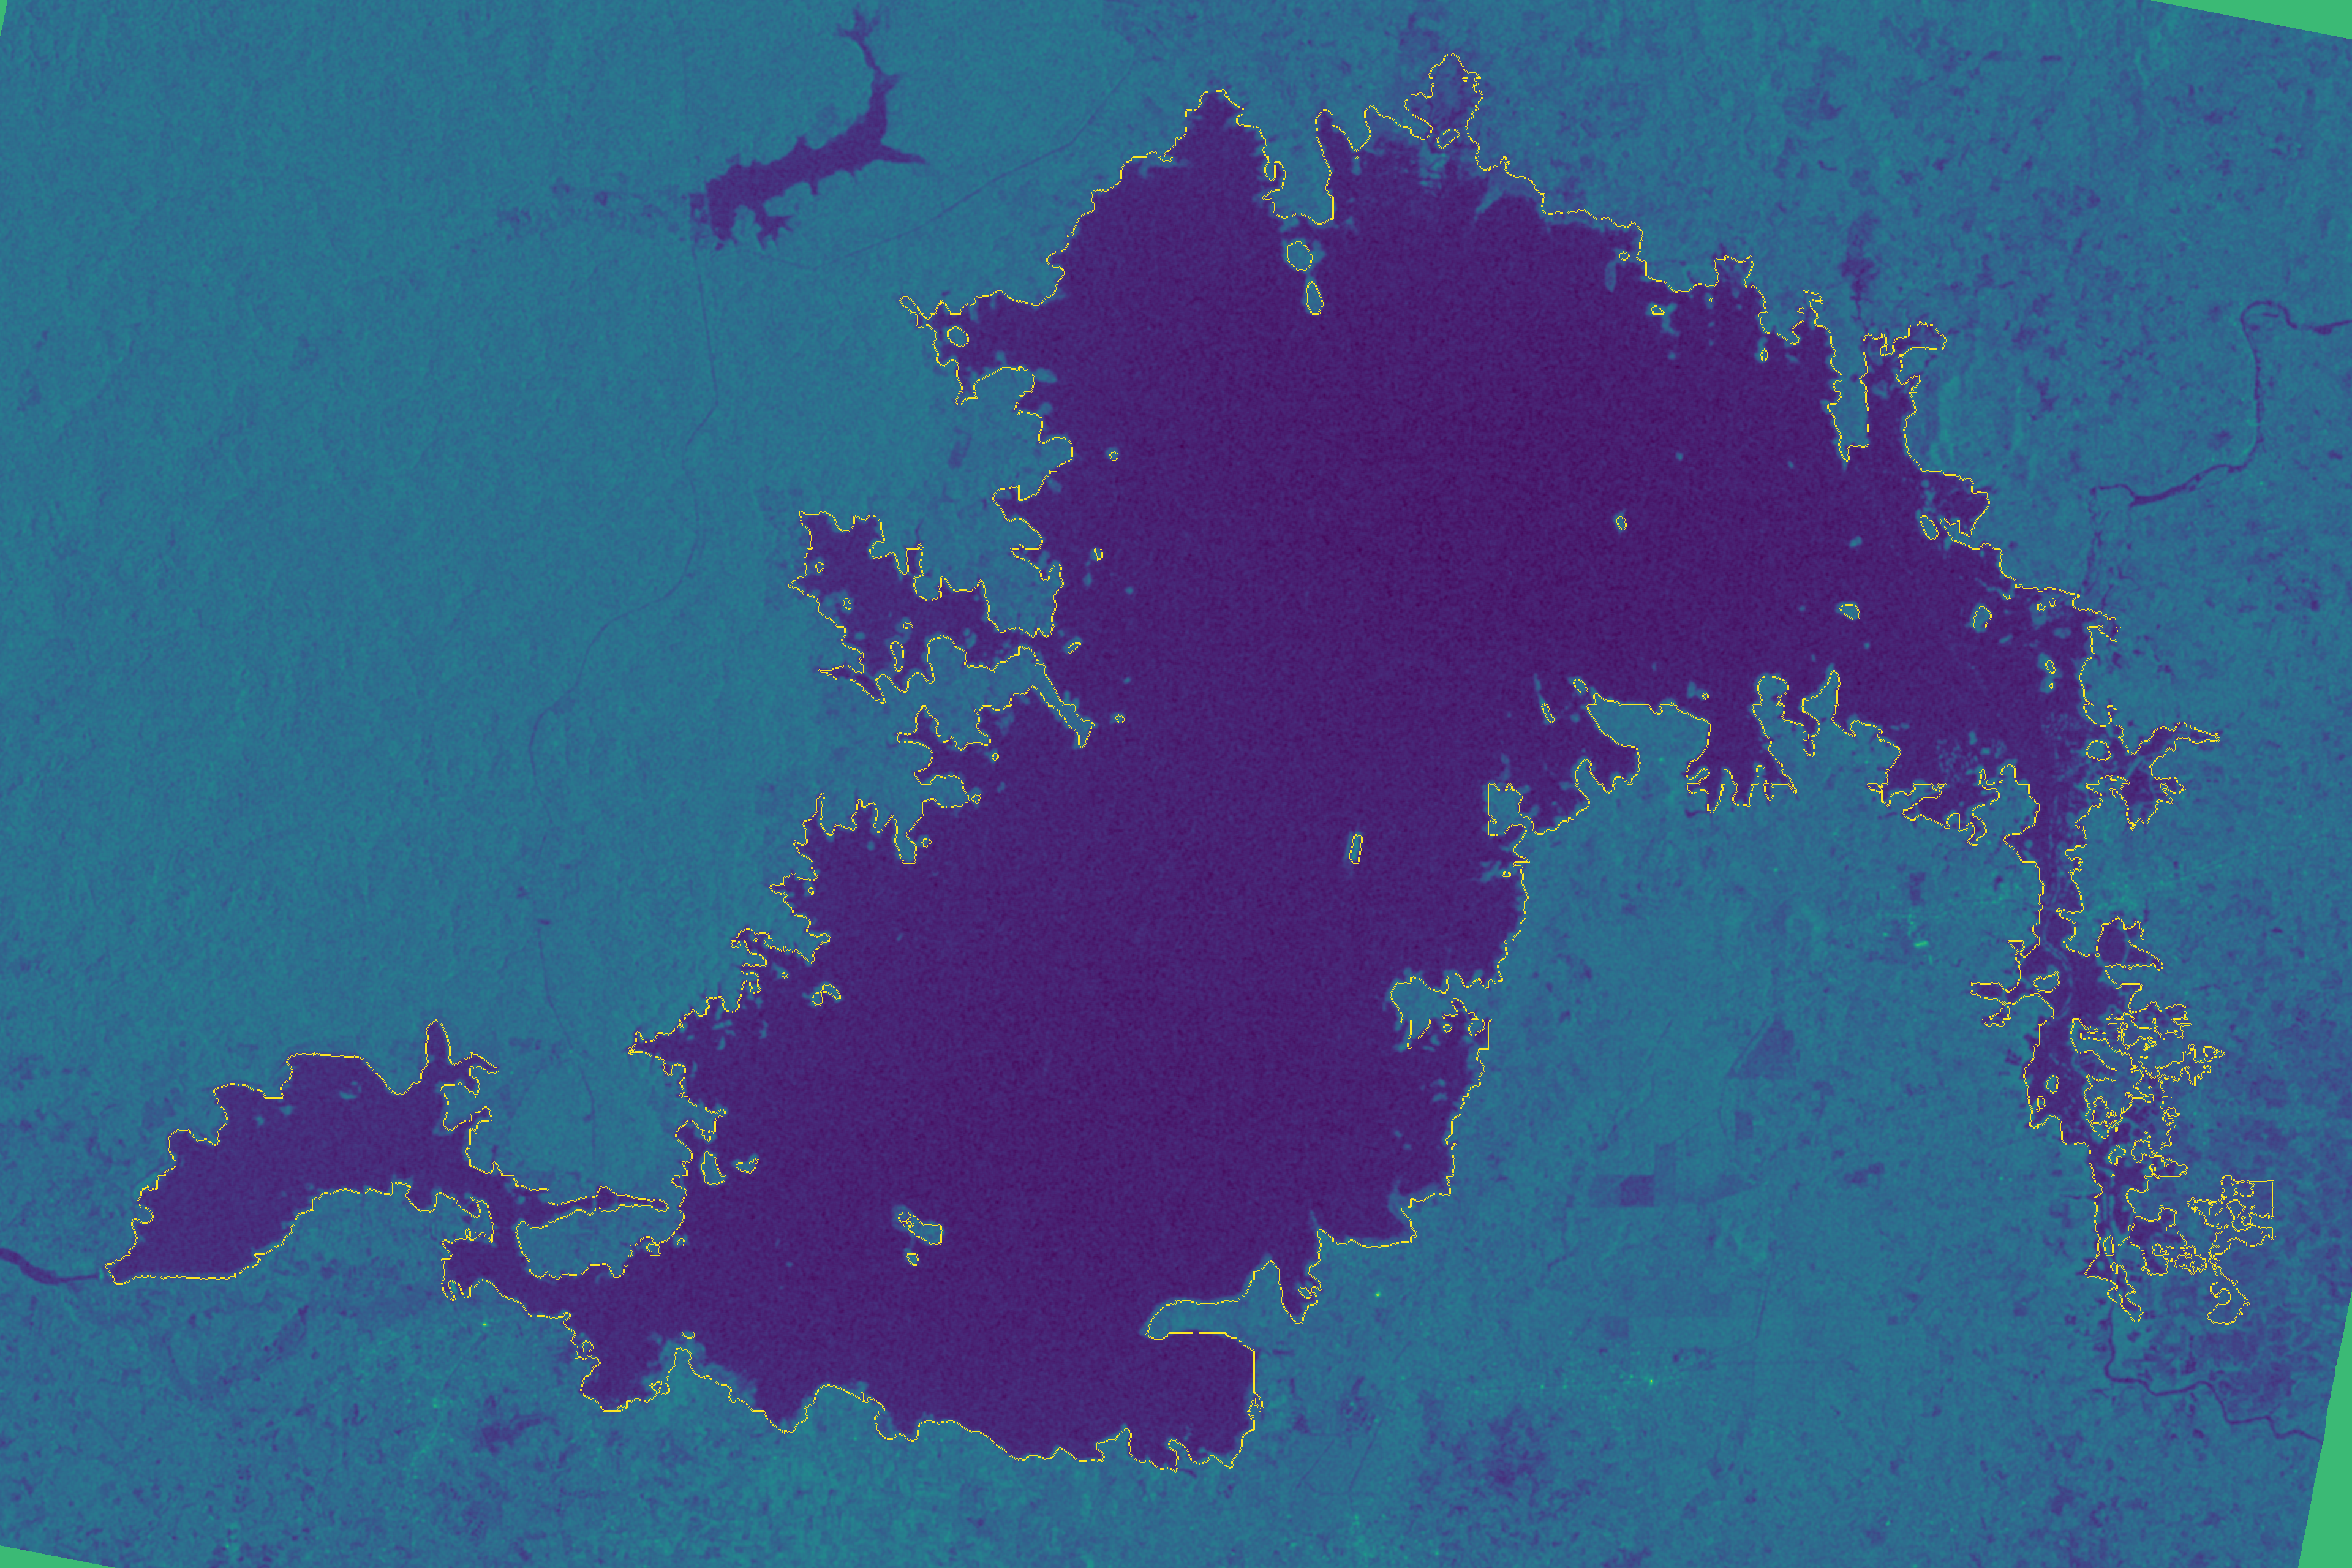
\includegraphics[width=0.9\textwidth]{figures/20190309T223707.png}
	\caption[]{Prediction, March 2019}
		\label{fig:prediction_03}
\end{figure}

\begin{figure}[h!]
	\centering
	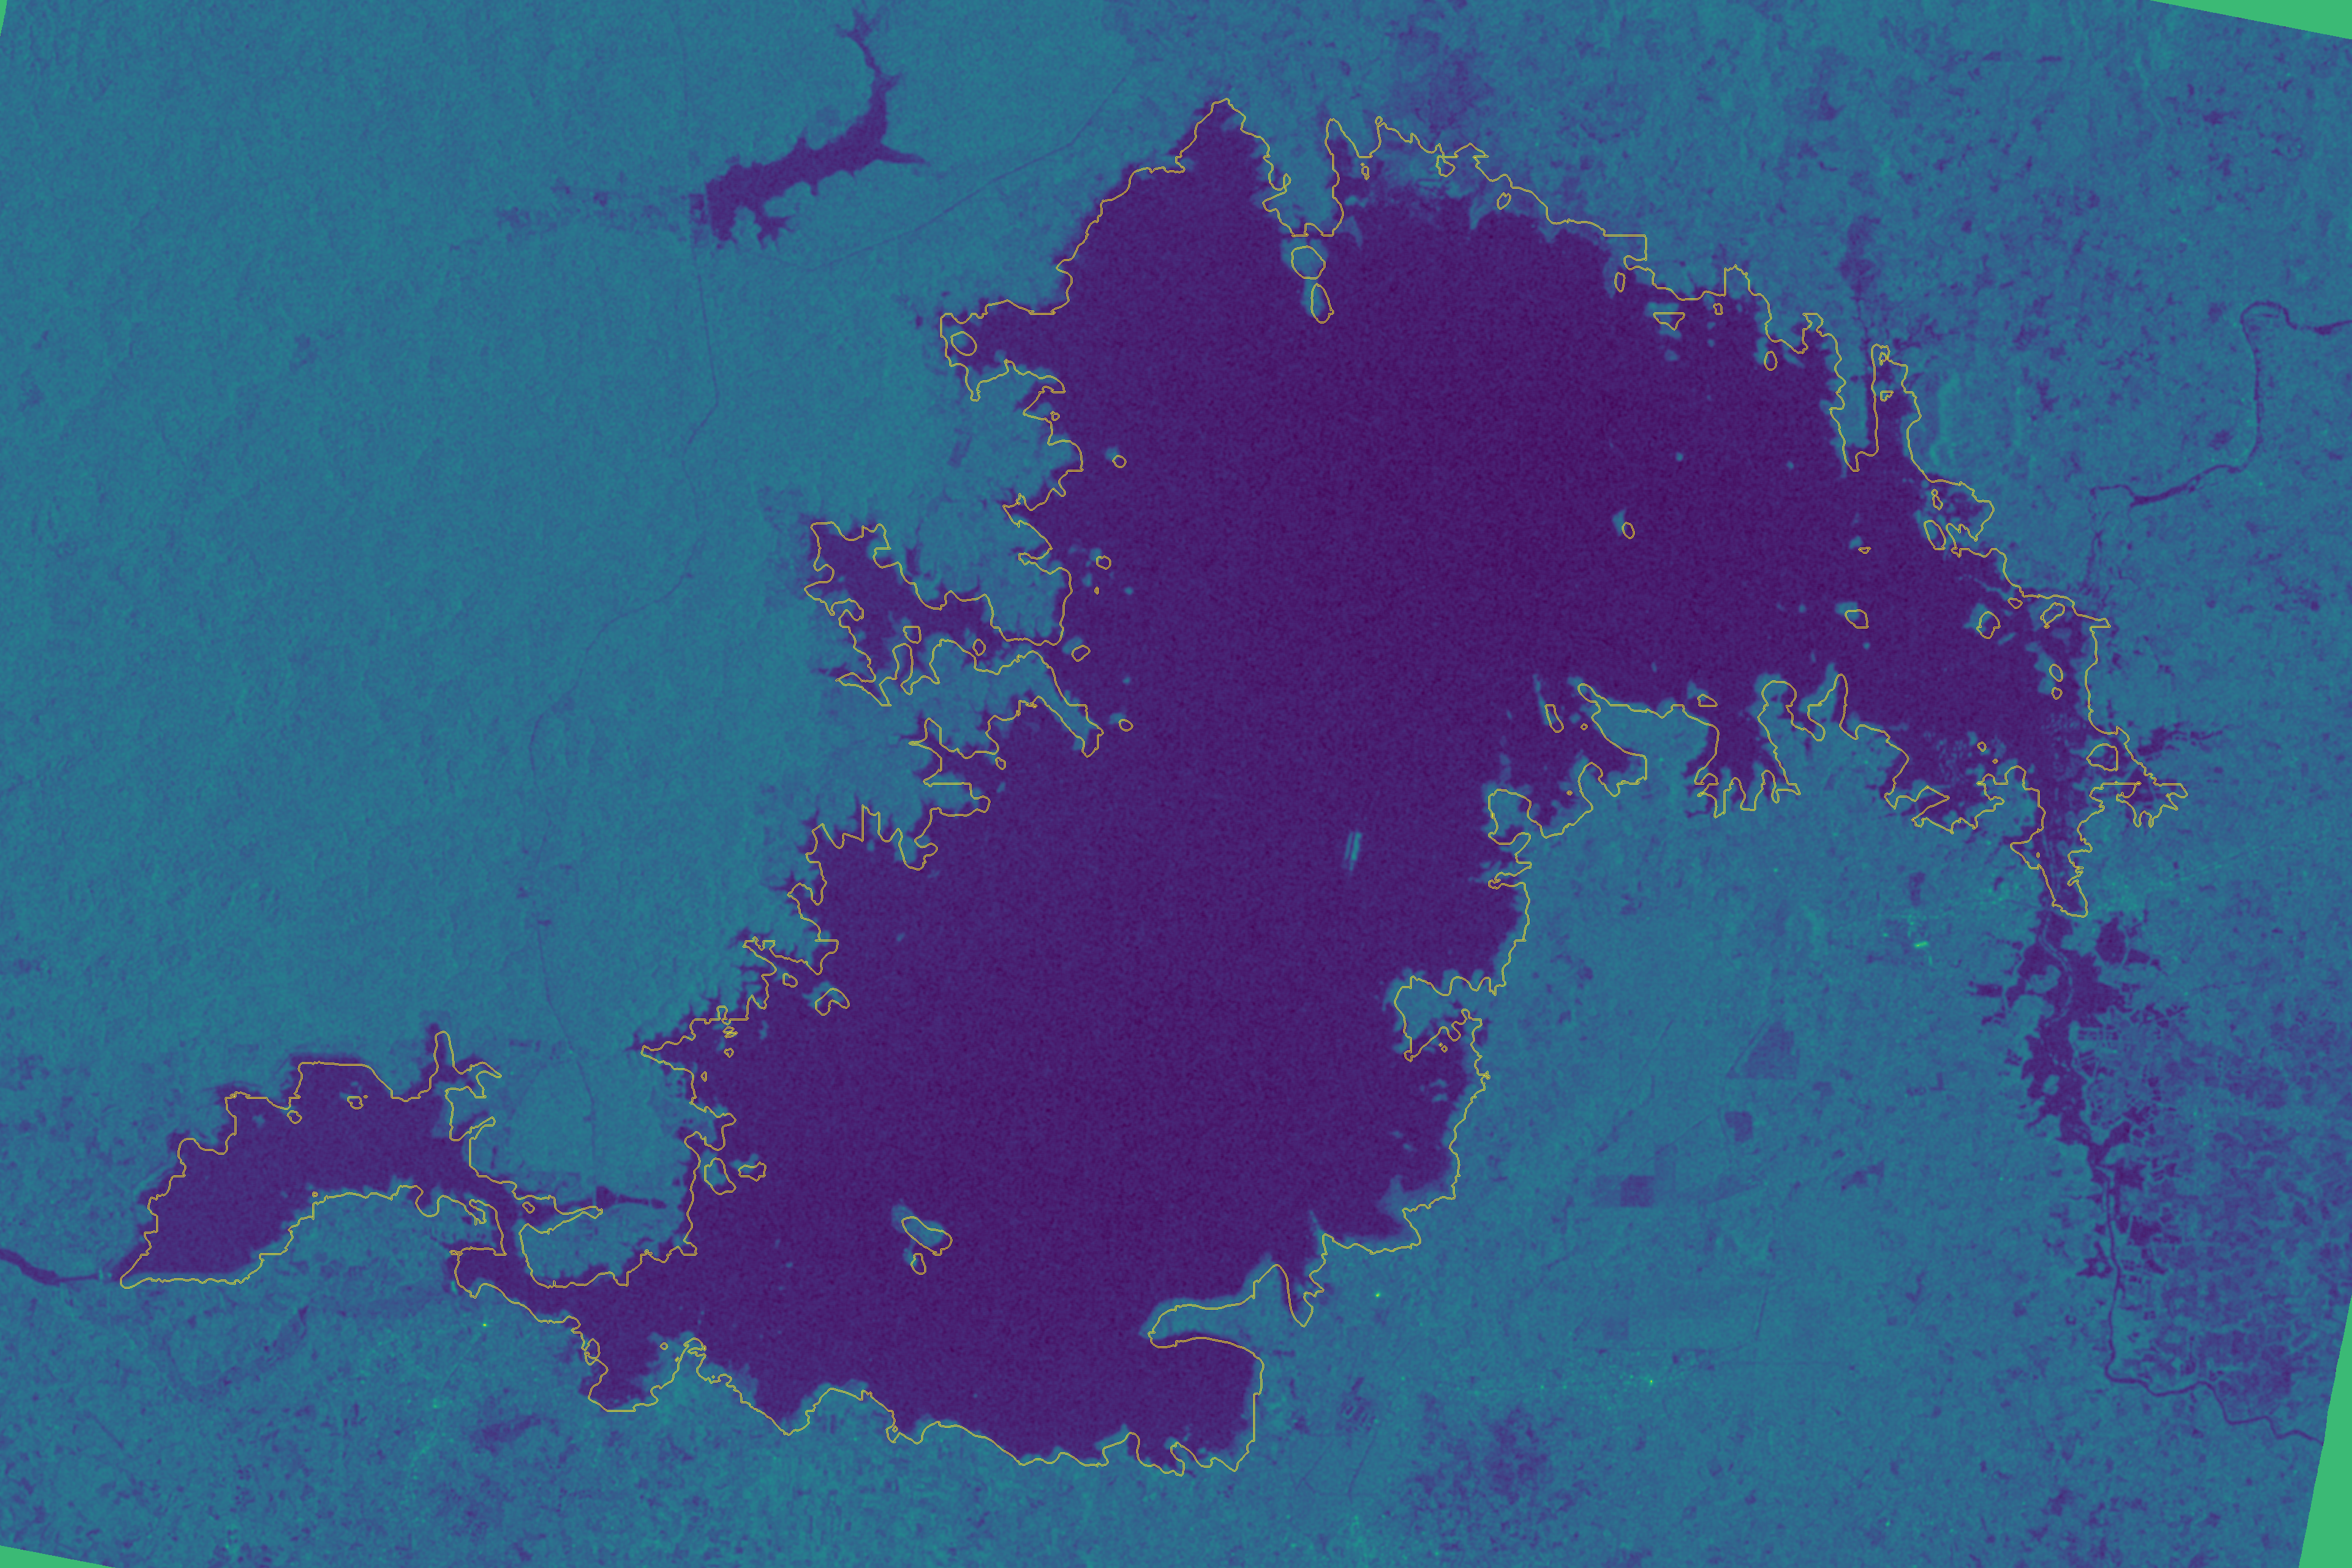
\includegraphics[width=0.9\textwidth]{figures/20190402T223708.png}
	\caption[]{Prediction, April 2019}
		\label{fig:prediction_04}
\end{figure}

\begin{figure}[h!]
	\centering
	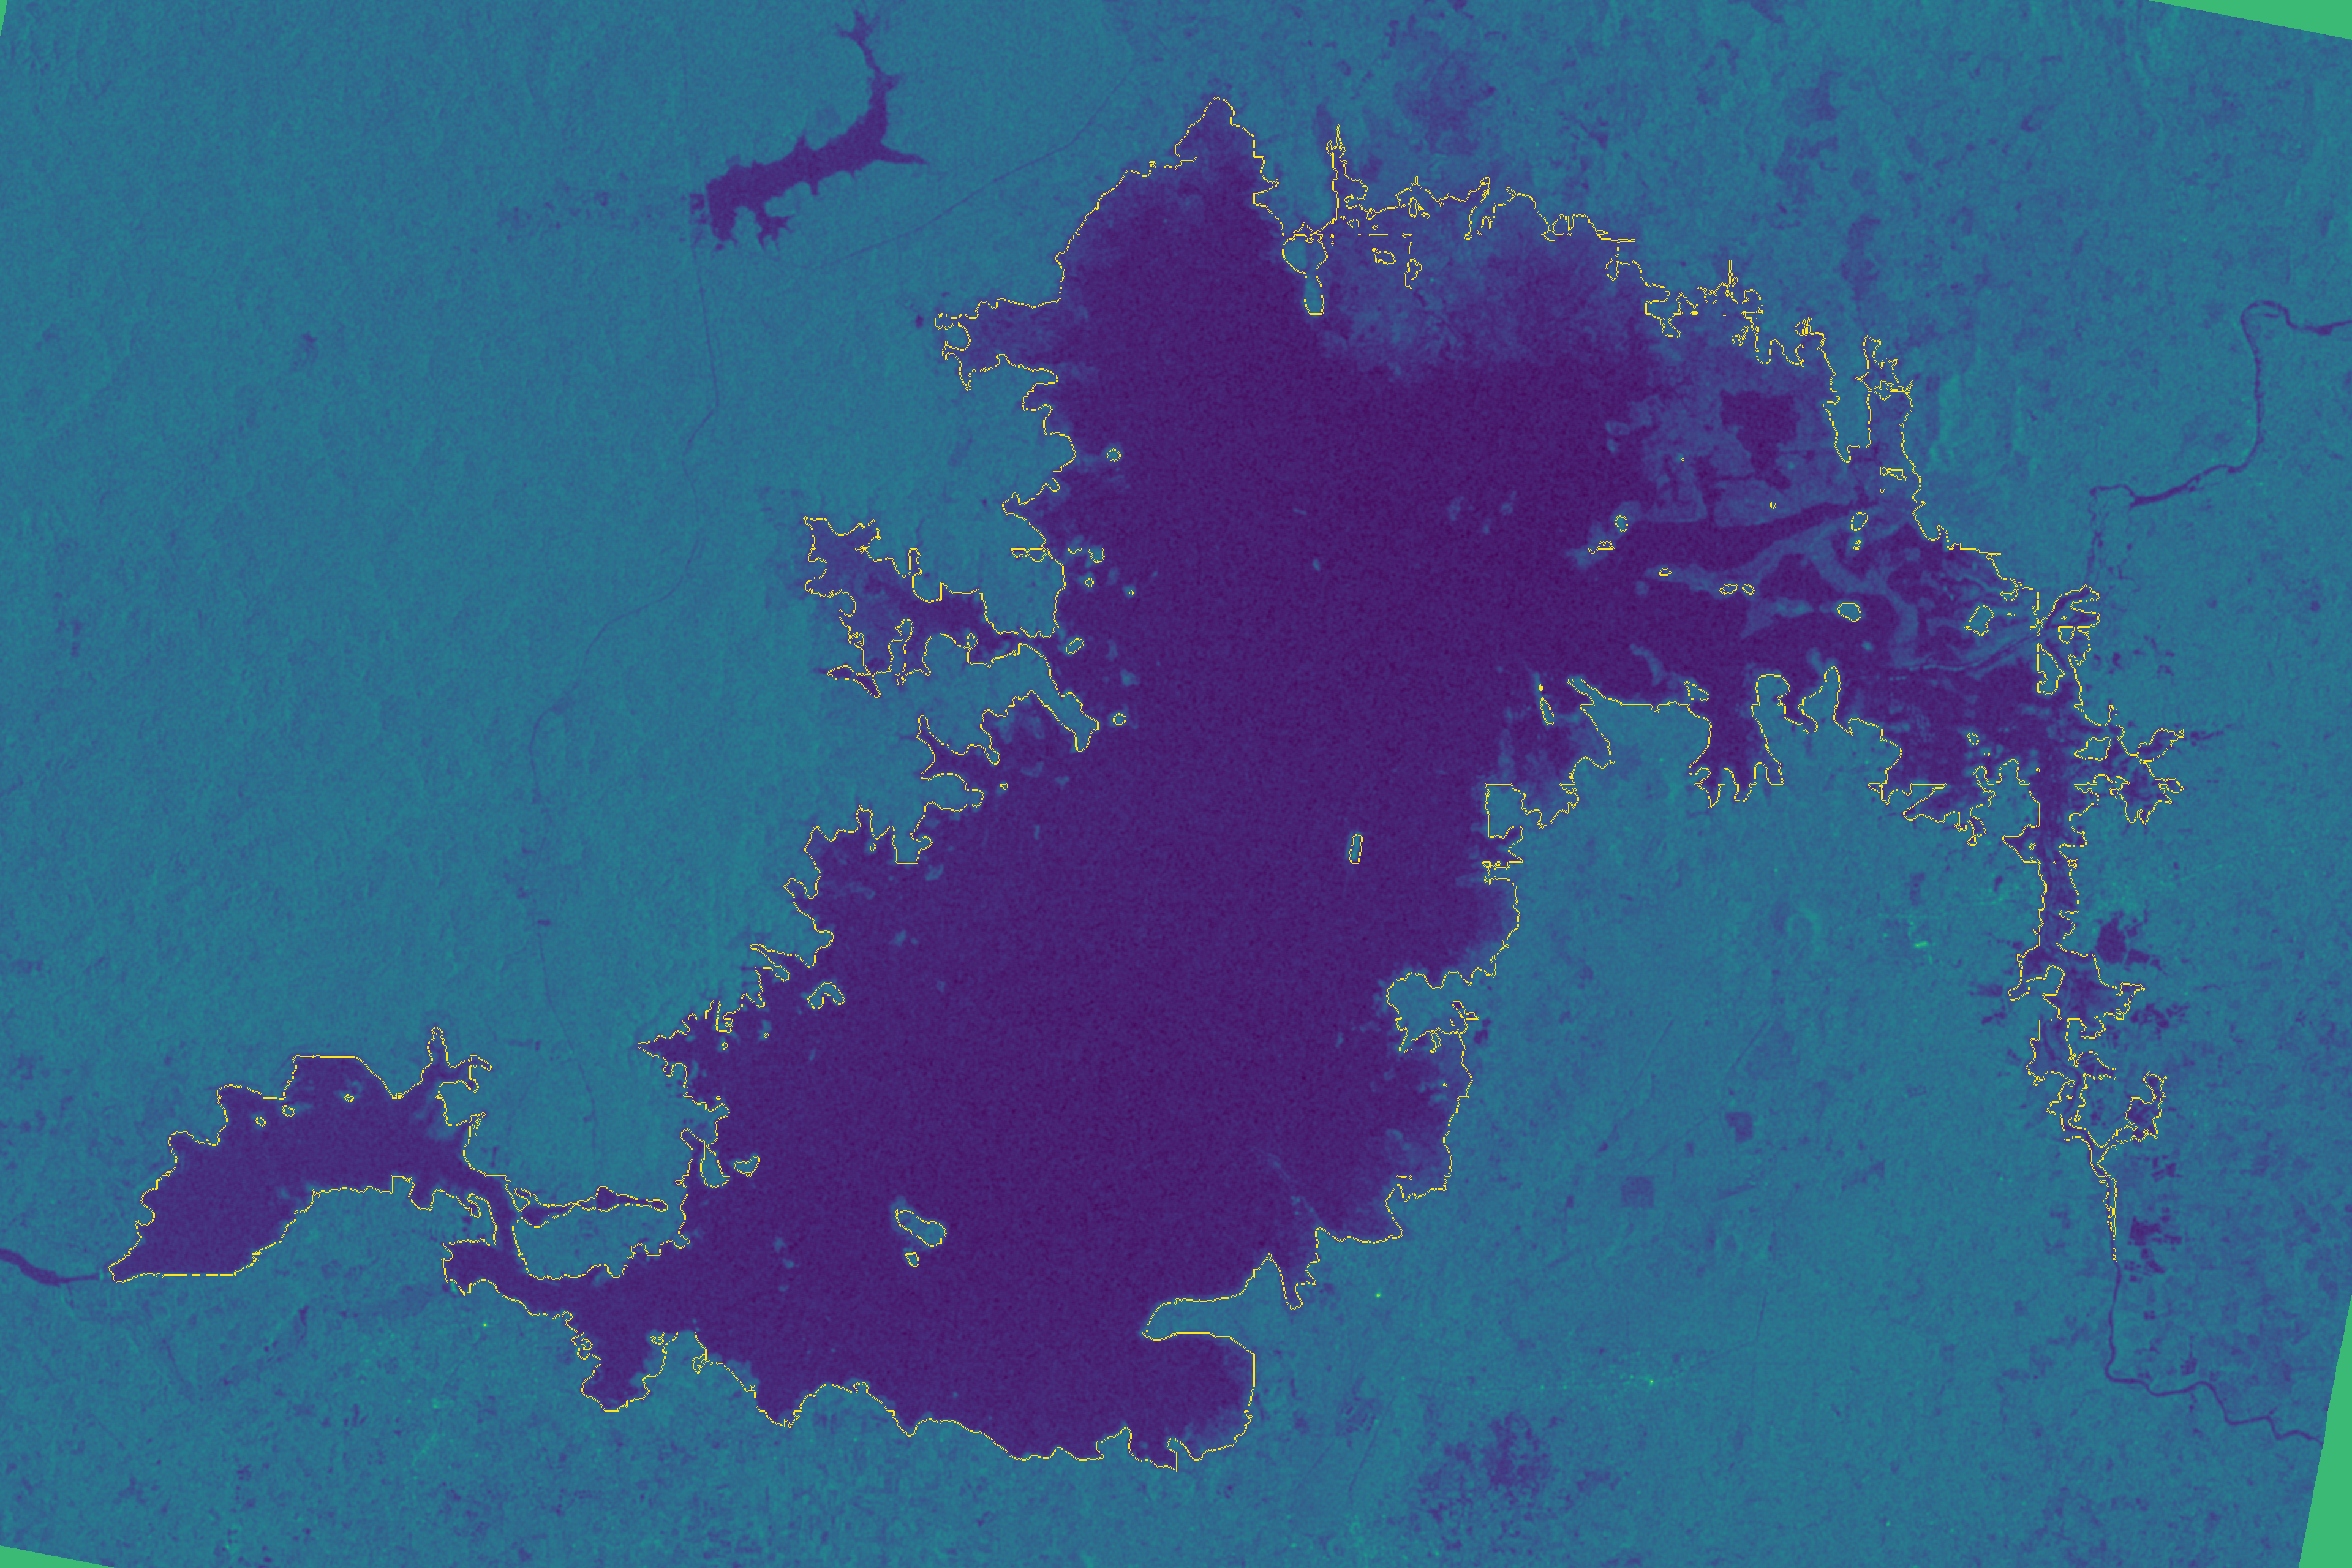
\includegraphics[width=0.9\textwidth]{figures/20190508T223709.png}
	\caption[]{Prediction, May 2019}
		\label{fig:prediction_05}
\end{figure}

\begin{figure}[h!]
	\centering
	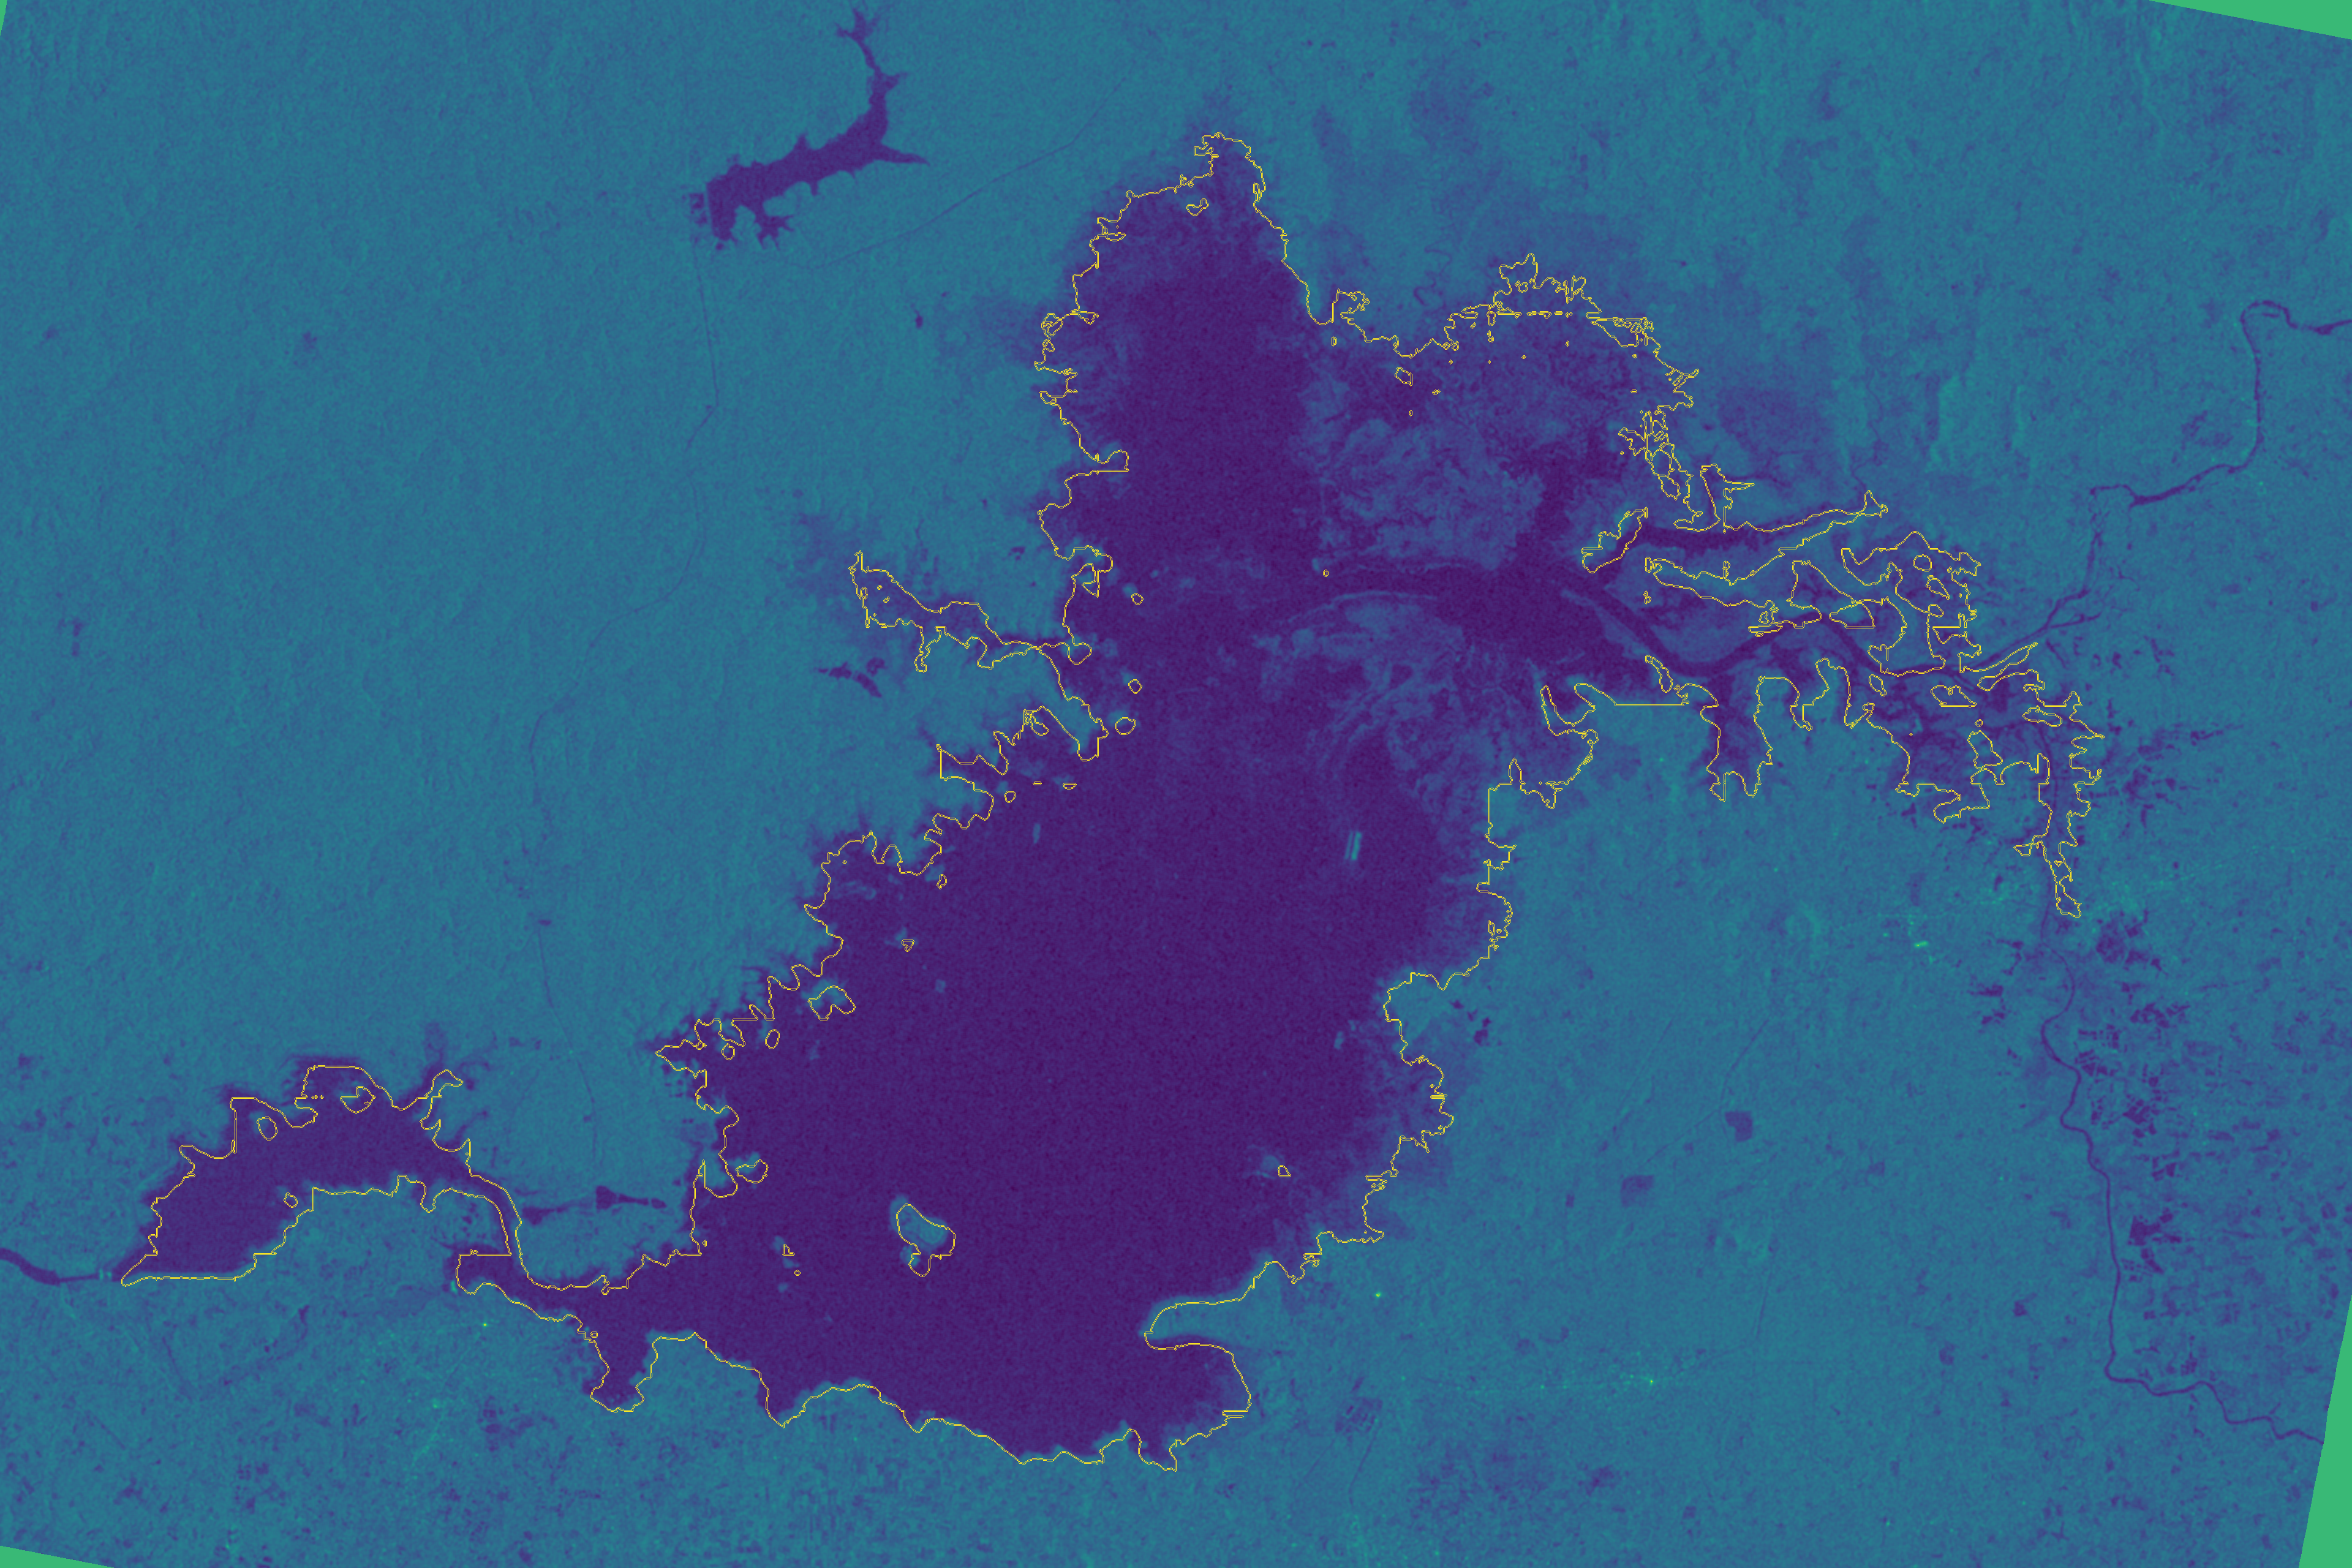
\includegraphics[width=0.9\textwidth]{figures/20190601T223710.png}
	\caption[]{Prediction, June 2019}
		\label{fig:prediction_06}
\end{figure}


\subsection{Example with anomaly detection}
\label{section:anomalyDetection}

One usage of sequence prediction output is about anomaly detection. This problem is usually formulated as finding outlier data points, relative to some standard or usual signal. In this chapter, the data points show water body area of Tri An Reservoir. The below chart show observations of Tri An reservoir area in 3 years, from 2016-2018.

\begin{figure}[h!]
	\centering
	\includegraphics[width=0.9\textwidth]{figures/observations.png}
	\caption[]{Observations of Tri An reservoir from Sentinel-1 Satellite, in term of water body area. Notice that, on July 2017, the water body area is seemed to be different from year 2016 and 2018}
	\label{fig:observation}
\end{figure}

Following observations, the groundtruth area of water body in 2016, 2017 and 2018 are $189.6926 km^2$, $242.4104 km^2$ and $178.4857 km^2$ respectively. While using our model, the prediction is approximately $189.6926 km^2$. See more about visualization at Fig. \ref{fig:anomalyVis} and graph for comparison at Fig. \ref{fig:anomalyComp}

\begin{figure}[h!]
	\centering
	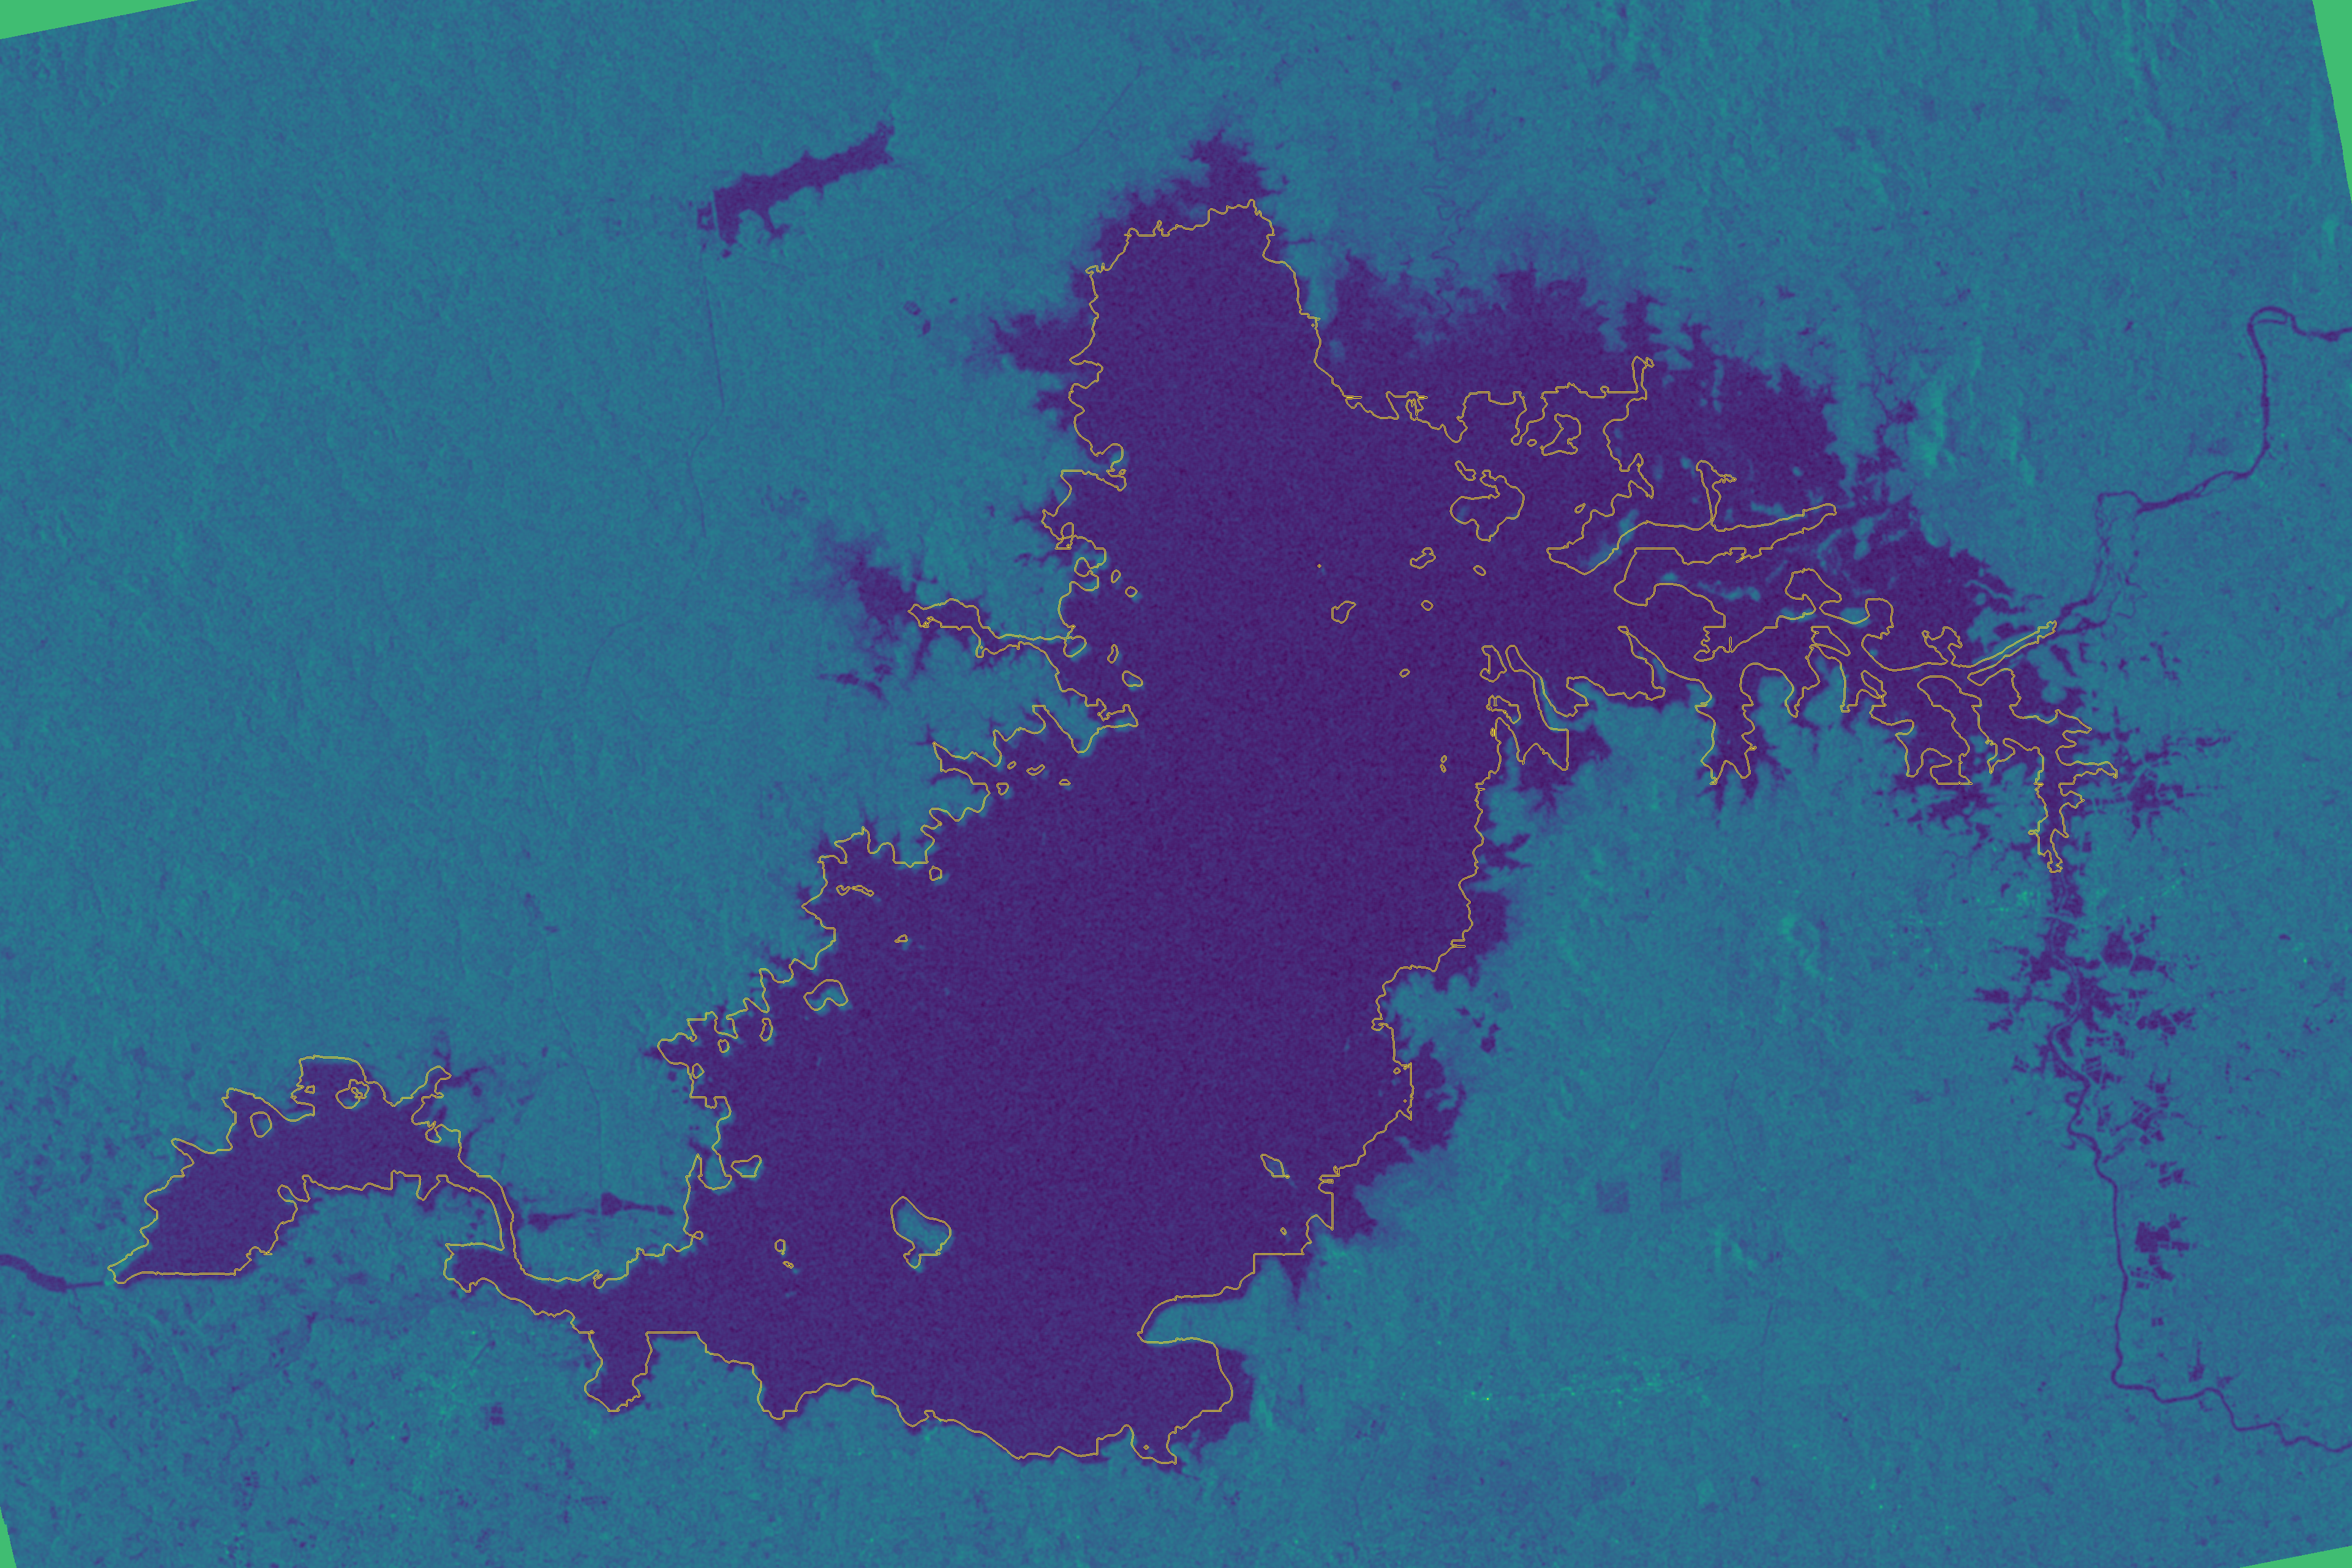
\includegraphics[width=0.9\textwidth]{figures/20170706T110259.png}
	\caption[]{Prediction for July 2017, using 12 previous data points (from July 2016 to Jun 2017)}
	\label{fig:anomalyVis}
\end{figure}


\begin{figure}[h!]
	\centering
	\includegraphics[width=0.9\textwidth]{figures/anomaly.png}
	\caption[]{Prediction (the red point) and groundtruth (the green line) on July 2017}
	\label{fig:anomalyComp}
\end{figure}

\section{Conclusions}

In this chapter, we have an acceptable result on applying deep learning to prediction problem on Tri An Reservoir, in term of water body area and its boundaries. This potential result may help us a lot when dealing with sequence prediction problem, especially complicated situation, such as spatial-temporal sequence forecasting problem, using proposed extension of LSTM - Conv-LSTM-2D. Beside that, with accepted prediction, the output of this problem may be used on other sequence problems, such as anomaly detection that we've taken example in \ref{section:anomalyDetection}. For future work, when enough data for training and testing, an end-to-end real-time forecasting water body observer system might be proposed, with two main parts: Prediction part and classification for anomalies part. 